% ============================================================
\section*{Materials and methods}
% ============================================================

The method is an extension of ULTRA \cite{bashir2026ultra}, not a second search engine. We keep the news corpus and the encoder. We change three things: what SHORT and LONG mean, which index is opened, and what the SVM probability is allowed to do.

\subsection*{System architecture}
\label{sec:architecture}

Fig~\ref{fig:architecture} is the old pipeline drawing from the development notebooks. Fig~\ref{fig:two_rooms} is the routing we actually evaluate. A query is normalized, scored by the SVM, and sent to a headline index, a full-article index, or a mix of both.

\begin{figure}[H]
\centering
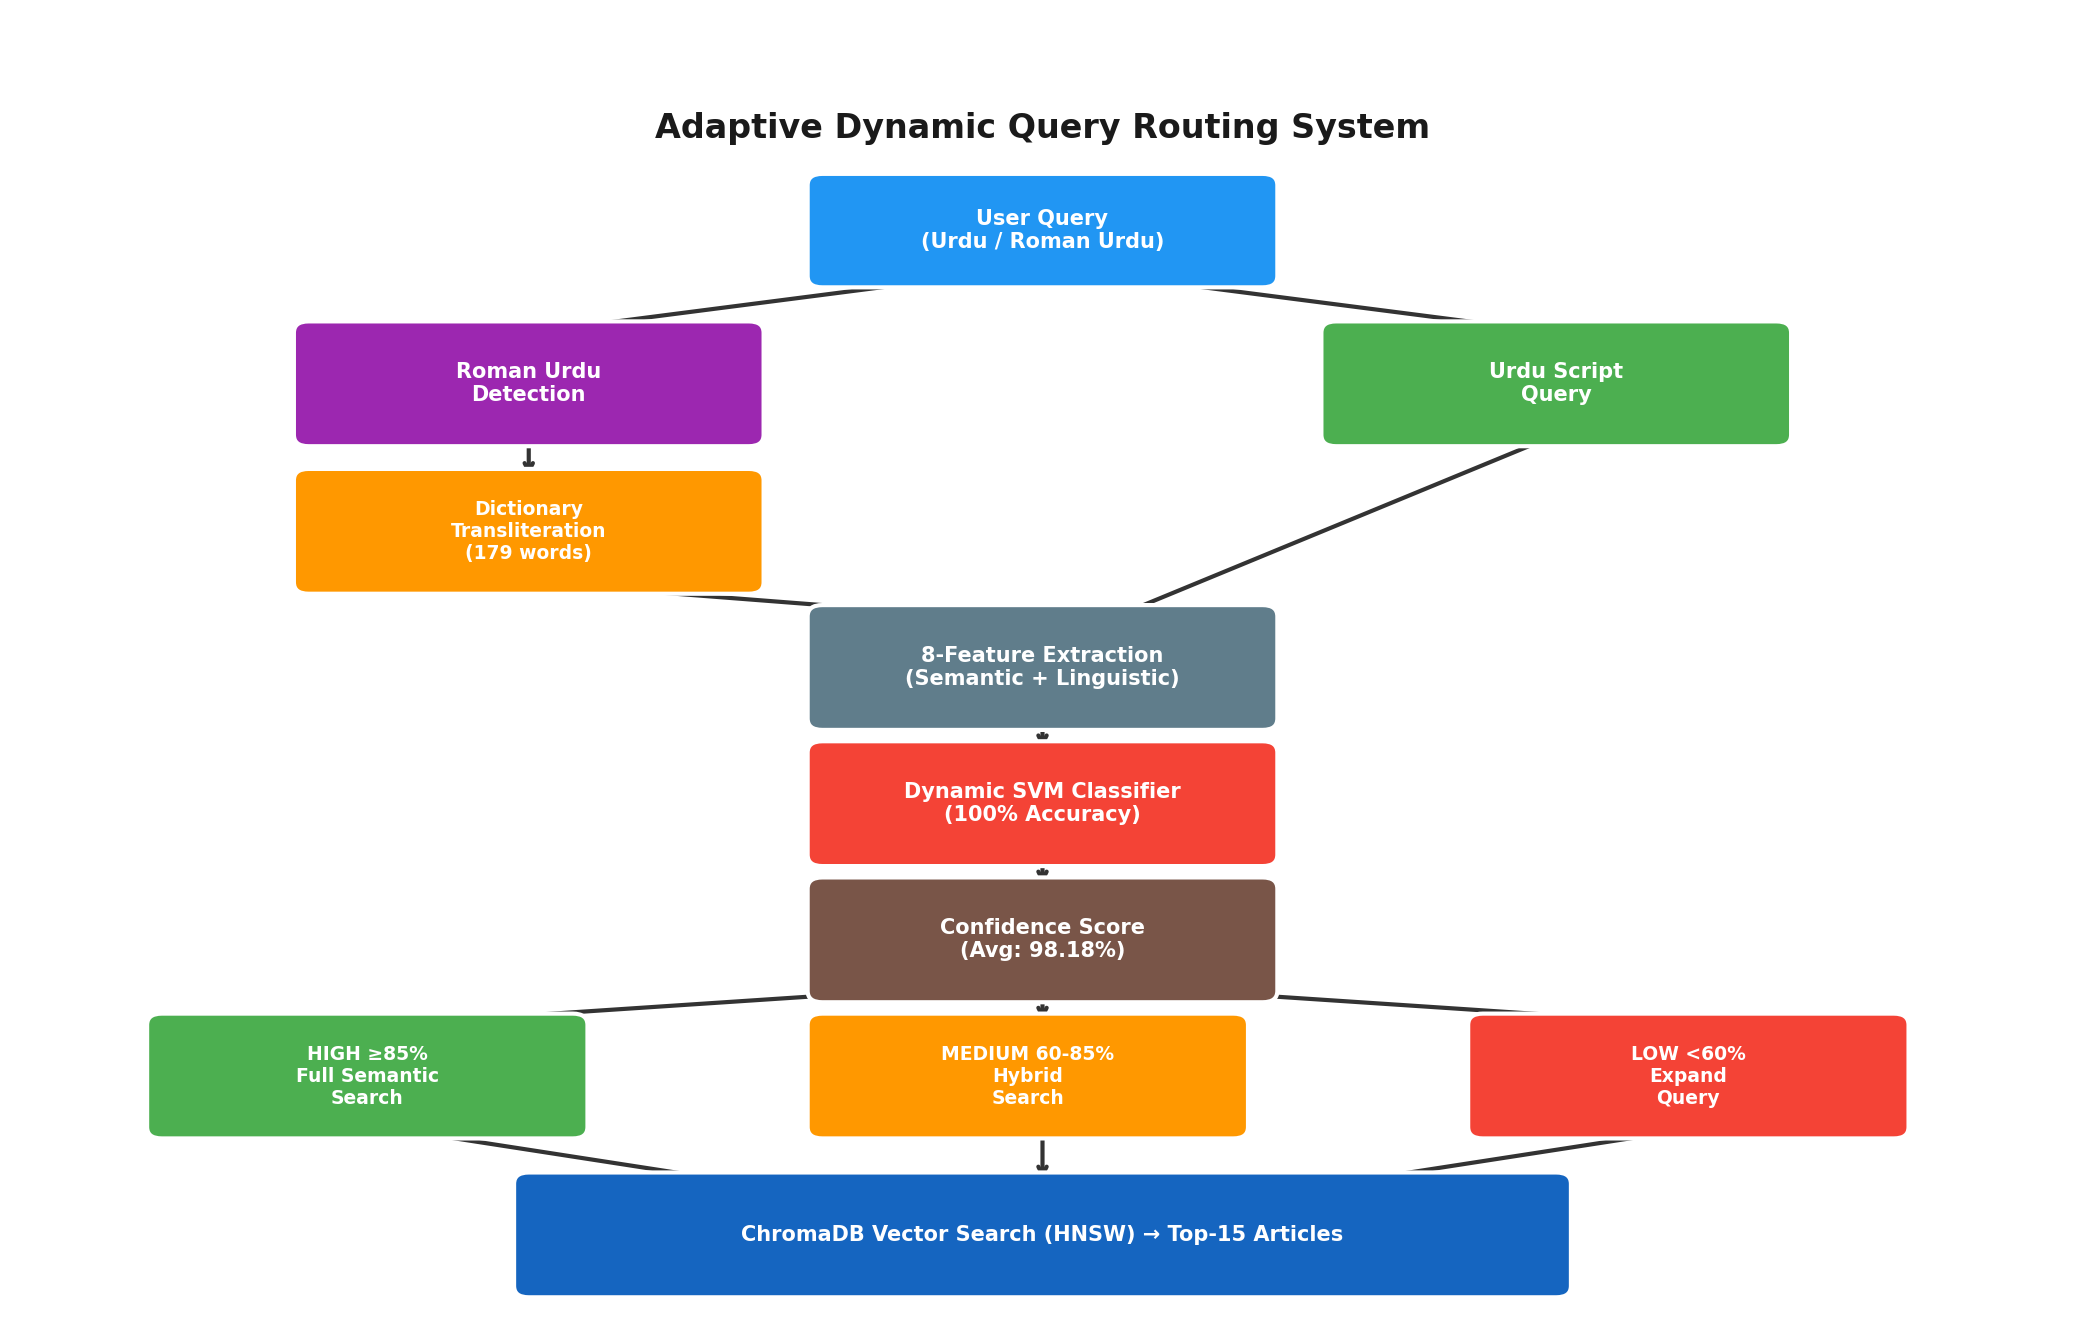
\includegraphics[width=\linewidth]{figures/system_architecture.png}
\caption{\textbf{Development pipeline diagram} (legacy notebook figure). Retrieval in the frozen tests uses two indexes, not a single Chroma search for every query. See Fig~\ref{fig:two_rooms}.}
\label{fig:architecture}
\end{figure}

\begin{figure}[H]
\centering
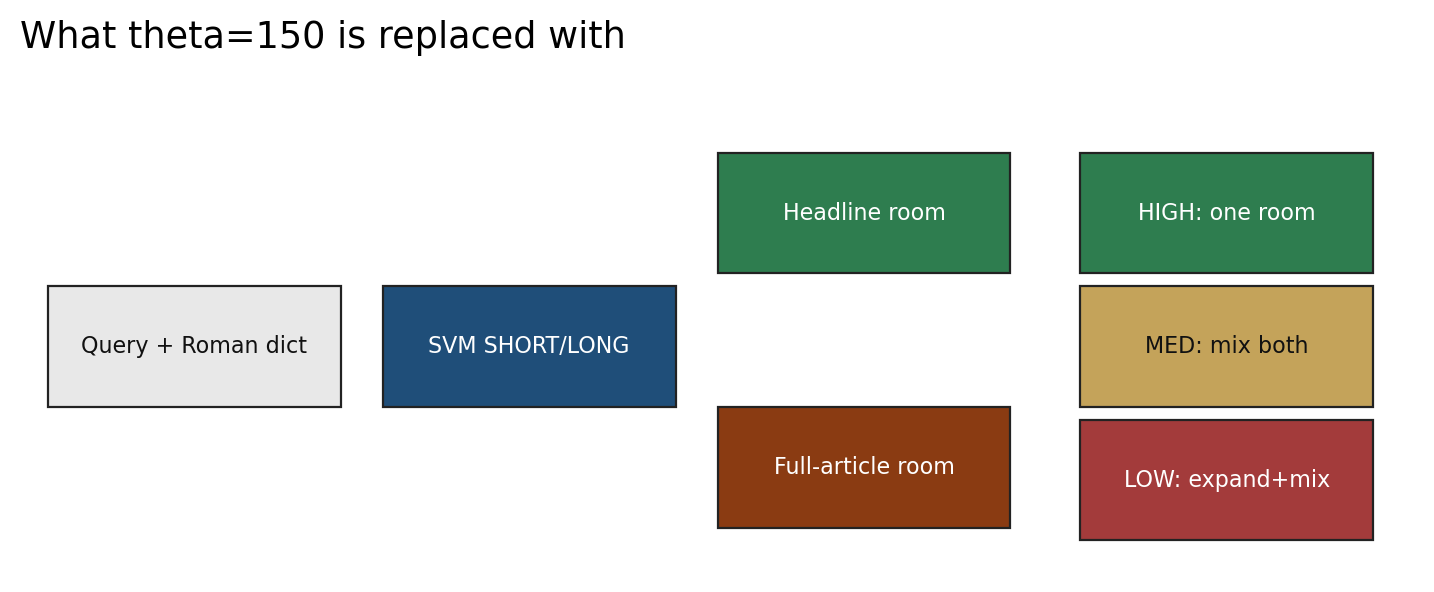
\includegraphics[width=\linewidth]{figures/two_rooms_lights.png}
\caption{\textbf{What the router actually does.} SHORT opens the headline room. LONG opens the full-article room. HIGH confidence stays in one room. MEDIUM mixes both. LOW expands the query and then mixes.}
\label{fig:two_rooms}
\end{figure}

Roman Urdu is mapped with a word list. The file on disk has 198 pairs (older drafts said 179). Native-script Urdu skips that step.

\subsection*{Corpus and indexes}
\label{sec:dataset}

The collection is 111,860 Urdu news articles (Kaggle Urdu News), embedded with \texttt{paraphrase-multilingual-MiniLM-L12-v2} \cite{reimers2019sbert} (384 dimensions) and stored in ChromaDB (\texttt{urdu\_news}) with HNSW and cosine similarity. That store is the full-article room. The headline room is a separate dense index over titles. Both rooms use the same encoder. We did not retrain it after seeing scores.

\begin{table}[H]
\centering
\caption{\textbf{Corpus category breakdown (111,860 articles).}}
\label{tab:corpus_categories}
\small
\begin{tabular}{lcc}
\toprule
\textbf{Category} & \textbf{Articles} & \textbf{\%} \\
\midrule
Sports & 44,829 & 40.07\% \\
Entertainment & 34,901 & 31.21\% \\
Business \& Economics & 24,131 & 21.57\% \\
Science \& Technology & 7,999 & 7.15\% \\
\bottomrule
\end{tabular}
\end{table}

Table~\ref{tab:dataset_summary} lists the query sets we actually freeze. They are not one pool.

\begin{table}[H]
\centering
\caption{\textbf{Query sets used in this paper. Do not average them.}}
\label{tab:dataset_summary}
\small
\begin{tabular}{p{4.2cm} p{6.2cm}}
\toprule
\textbf{Set} & \textbf{Role} \\
\midrule
Development / CV (369--409 labeled queries) & Shows the task is learnable. Some splits hit 100\% vs 50\% for $\theta=150$. Not the paper headline. \\
Frozen Phase 3B, V2, 8 features & 50 primary queries. SVM 86\% vs word count $\geq 6$ at 84\%. \\
Frozen traps H001--H040 & Need labels. Never used to train V2. Classification and dual-index P@5. \\
Phase 2.5 & 33 queries, P@5 depth 5. Supporting only. \\
Roman Urdu dictionary & 198 pairs on disk. \\
\bottomrule
\end{tabular}
\end{table}

Fig~\ref{fig:query_dist} is the development length plot. It still makes the basic point: almost nothing reaches 150 characters, so $\theta=150$ is a dead switch on this query mix.

\begin{figure}[H]
\centering
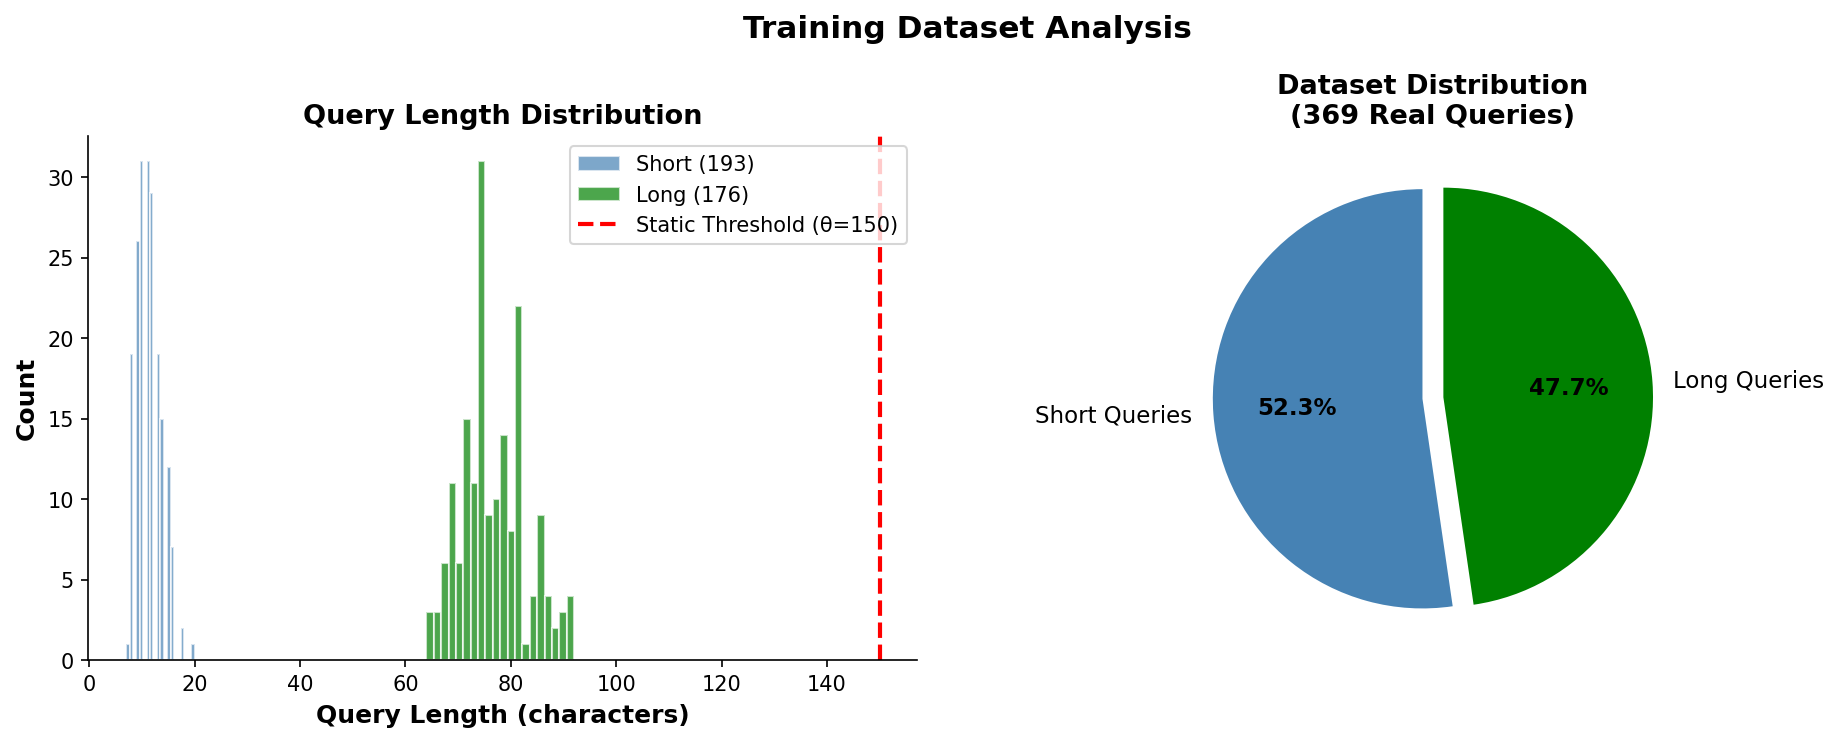
\includegraphics[width=\linewidth]{figures/query_distribution.png}
\caption{\textbf{Development query lengths vs.\ $\theta=150$.} Most queries sit well below the cutoff. That is why the static rule collapses to SHORT.}
\label{fig:query_dist}
\end{figure}

\subsection*{What SHORT and LONG mean}
\label{sec:labels}

SHORT means a headline could answer the user (score, price, date, who won). LONG means they asked for why, how, impact, or a story. We did not label by token count. If we had, we could never beat a six-word rule.

\subsection*{Eight-feature SVM (frozen V2)}
\label{sec:features}

The frozen generalization model uses eight features:

\begin{equation}
\mathbf{x}(q) = \big[x_1(q),\ldots,x_8(q)\big] \in \mathbb{R}^{8}
\label{eq:featurevec}
\end{equation}

\begin{table}[H]
\centering
\caption{\textbf{Frozen V2 feature vector (Phase 3B).}}
\label{tab:features}
\small
\begin{tabular}{clp{4.2cm}}
\toprule
\textbf{\#} & \textbf{Feature} & \textbf{Definition} \\
\midrule
$x_1$ & \texttt{urdu\_ratio} & Share of Urdu-script characters \\
$x_2$ & \texttt{roman\_ratio} & Share of Latin-script characters \\
$x_3$ & \texttt{has\_urdu} & Binary: any Urdu character \\
$x_4$ & \texttt{has\_roman} & Binary: any Latin letter \\
$x_5$ & \texttt{query\_len} & Whitespace token count \\
$x_6$ & \texttt{char\_len} & Character count \\
$x_7$ & \texttt{mixed} & Both scripts present \\
$x_8$ & \texttt{urdu\_chars} & Count of Urdu characters \\
\bottomrule
\end{tabular}
\end{table}

Features are z-scored on the training split only \cite{cortes1995svm}. The SVM uses an RBF kernel. Class probability is Platt scaling \cite{guo2017calibration}:

\begin{equation}
C(q) = \sigma\big(A f(\mathbf{z}(q)) + B\big) \times 100\%
\label{eq:confidence}
\end{equation}

A later twelve-feature pickle exists in the demo. It is not the Phase 3B scorer. Mixing the two is how a 96\% figure appears. We do not report 96\%.

\subsection*{Lights, then rooms}
\label{sec:tiered_routing}

\begin{equation}
R(q) =
\begin{cases}
\text{chosen room only}, & C(q) \geq 85\% \quad \text{(HIGH)} \\[4pt]
\text{mix both rooms}, & 60\% \leq C(q) < 85\% \quad \text{(MEDIUM)} \\[4pt]
\text{expand, then mix}, & C(q) < 60\% \quad \text{(LOW)}
\end{cases}
\label{eq:routing}
\end{equation}

\begin{table}[H]
\centering
\caption{\textbf{Confidence lights.}}
\label{tab:routing_tiers}
\small
\begin{tabular}{llp{5.2cm}}
\toprule
\textbf{Light} & \textbf{$C(q)$} & \textbf{Search} \\
\midrule
HIGH & $\geq 85\%$ & Headline room if SHORT, full-article room if LONG \\
MEDIUM & $60$--$85\%$ & Mix both rooms \\
LOW & $< 60\%$ & Expand query, then mix \\
\bottomrule
\end{tabular}
\end{table}

LOW is implemented. On the small live probe we used for defense it did not fire. We do not pretend that it did.

Similarity in each room is cosine on MiniLM vectors, same as ULTRA's backend:

\begin{equation}
\mathrm{sim}(\mathbf{e}_q, \mathbf{e}_d)
= \frac{\mathbf{e}_q \cdot \mathbf{e}_d}{\lVert\mathbf{e}_q\rVert\,\lVert\mathbf{e}_d\rVert}.
\label{eq:cosine}
\end{equation}

\subsection*{Baselines}
\label{sec:baselines}

Frozen comparisons: $\theta=150$; word count $\geq 6$ tokens $\rightarrow$ LONG; always-headline; always-full-article; the V2 SVM. Development notebooks also compared LLM-style routers on 14 queries. Those numbers stay in the development layer. They are not frozen P@5.

\subsection*{Evaluation}
\label{sec:eval_metrics}

Classification: accuracy and exact McNemar tests. Retrieval: P@5 and nDCG@5 on 400 graded judgments (40 queries $\times$ 5). Phase 2.5 used 33 queries at depth 5. We do not convert a McNemar $p=1$ into a win speech.

\begin{figure}[H]
\centering
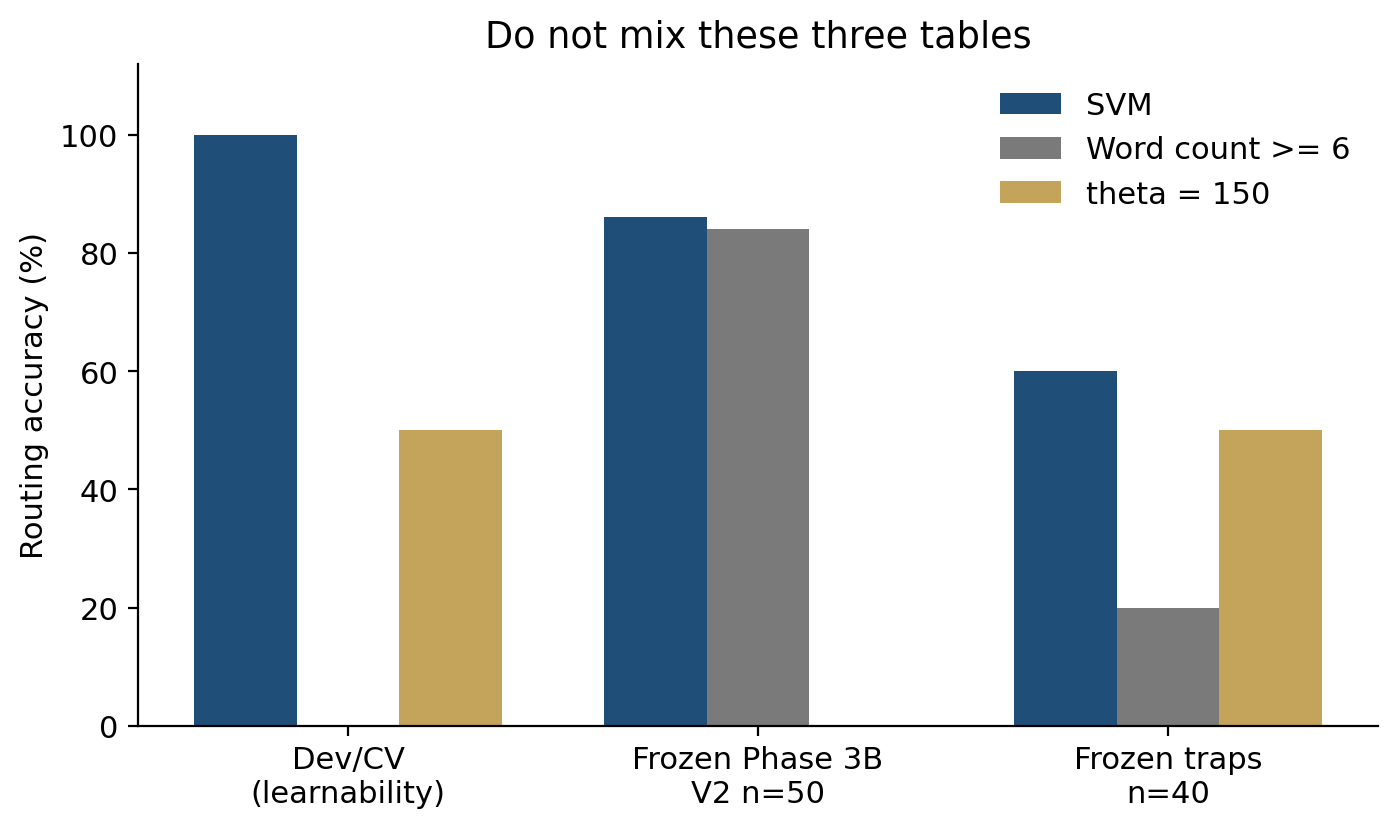
\includegraphics[width=\linewidth]{figures/three_evaluation_layers.png}
\caption{\textbf{Three layers that must not be mixed:} development/CV, frozen Phase 3B (86/84), frozen traps (60/20/50 and P@5).}
\label{fig:layers}
\end{figure}

% ============================================================
\section*{Results}
\label{sec:results}
% ============================================================

\subsection*{Development routing looks solved. That is not the claim.}
\label{sec:res_accuracy}

On development splits the SVM can hit 100\% while $\theta=150$ sits at 50\% (Table~\ref{tab:routing_accuracy}, Fig~\ref{fig:confusion_matrix}). Fig~\ref{fig:perf_comparison} is from that same notebook era. We keep the figures because they show learnability. We do not keep them as the generalization headline.

\begin{table}[H]
\centering
\caption{\textbf{Development routing accuracy (not frozen Phase 3B).}}
\label{tab:routing_accuracy}
\small
\begin{tabular}{lc}
\toprule
\textbf{Method} & \textbf{Accuracy} \\
\midrule
Static threshold ($\theta=150$) & 50.00\% \\
Logistic regression (dev split) & 100.00\% \\
SVM, RBF (dev split) & 100.00\% \\
\bottomrule
\end{tabular}
\end{table}

\begin{figure}[H]
\centering
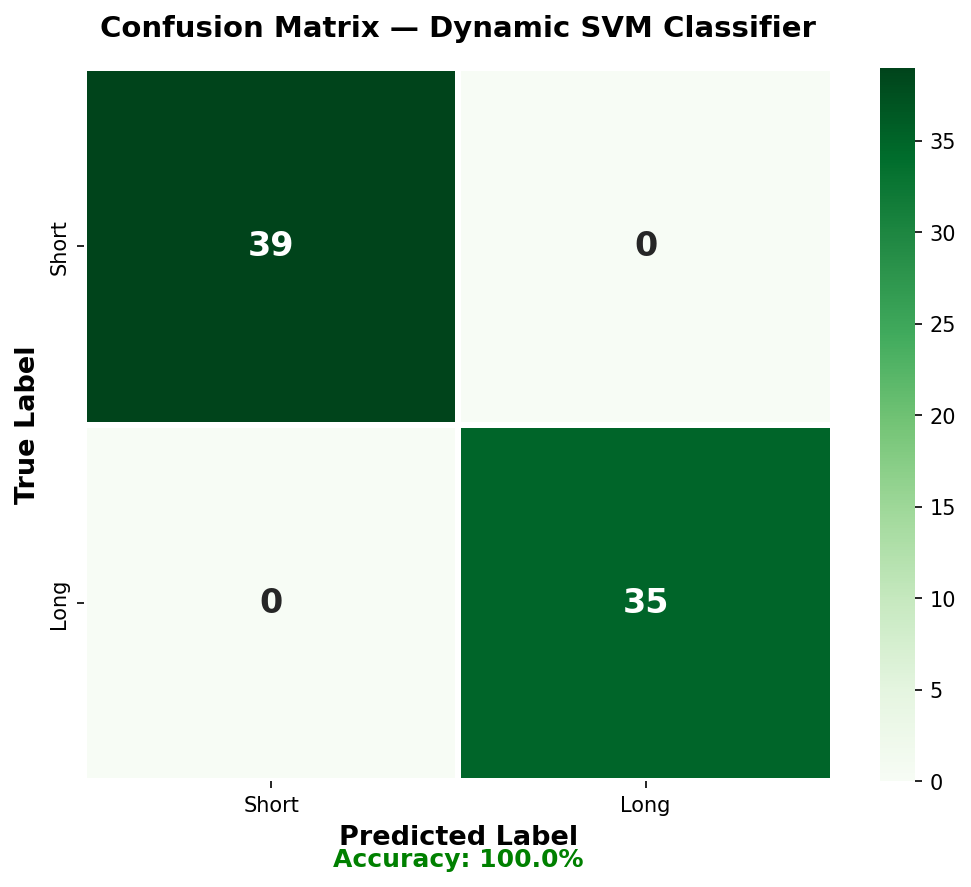
\includegraphics[width=\linewidth]{figures/confusion_matrix.png}
\caption{\textbf{Development confusion matrix} (74-query split). Treat as learnability, not as the frozen test.}
\label{fig:confusion_matrix}
\end{figure}

\begin{figure}[H]
\centering
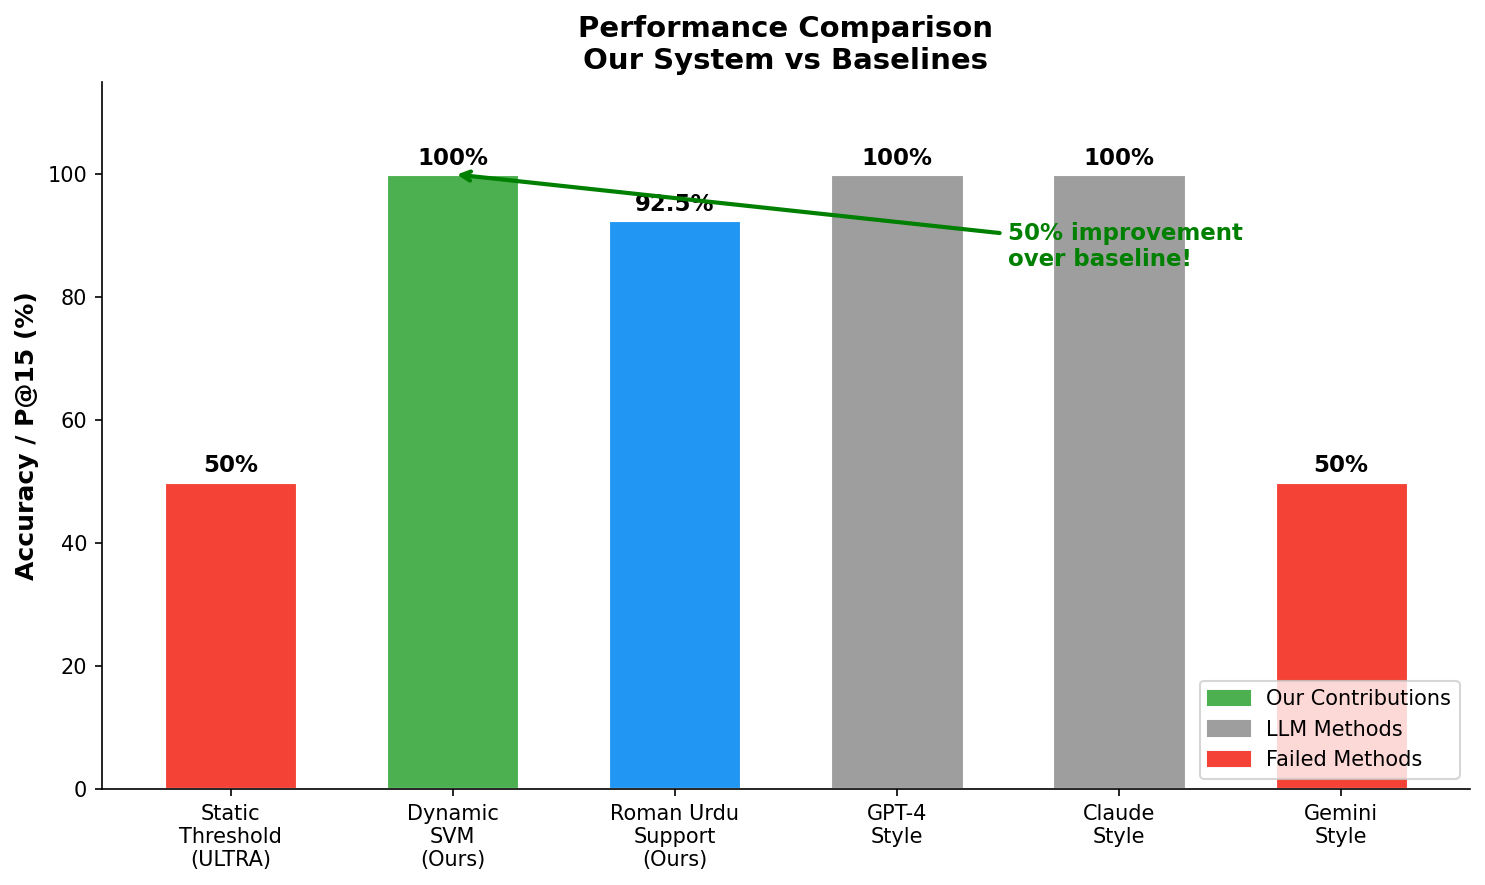
\includegraphics[width=\linewidth]{figures/performance_comparison.png}
\caption{\textbf{Development performance panel.} Do not quote this as the held-out result.}
\label{fig:perf_comparison}
\end{figure}

\subsection*{Frozen Phase 3B: 86\% vs 84\%}
\label{sec:res_p15}

On 50 primary queries the V2 SVM was right 43 times (86\%). Word count was right 42 times (84\%). McNemar is 2 vs 1, exact $p=1.0$. If this were the only experiment, the paper would be thin. It is a check that the frozen extractor matches the trained V2 model.

\subsection*{Frozen traps: a classification gap, with a catch}
\label{sec:res_traps}

On H001--H040 the SVM reached 60\%, word count 20\%, $\theta=150$ 50\%. McNemar vs word count is 16--0 ($p<0.001$).

The cue split is the part that should stay on the slide (Fig~\ref{fig:cue}). Eighteen queries fire why/how/fact wording: SVM 18/18, word count 2/18. The other 22 do not fire those cues: both systems 27.27\%. So the trap win is not ``the SVM understands need.'' It is ``the SVM notices certain words, and the traps were rich in those words.''

\begin{table}[H]
\centering
\caption{\textbf{Frozen classification. Do not mix with development 100\%.}}
\label{tab:frozen_cls}
\small
\begin{tabular}{lccc}
\toprule
\textbf{Layer} & \textbf{SVM} & \textbf{Word count} & \textbf{$\theta=150$} \\
\midrule
Phase 3B ($n=50$) & 86\% & 84\% & -- \\
Traps ($n=40$) & 60\% & 20\% & 50\% \\
Traps with cue ($n=18$) & 100\% & 11.11\% & -- \\
Traps, no cue ($n=22$) & 27.27\% & 27.27\% & -- \\
\bottomrule
\end{tabular}
\end{table}

\begin{figure}[H]
\centering
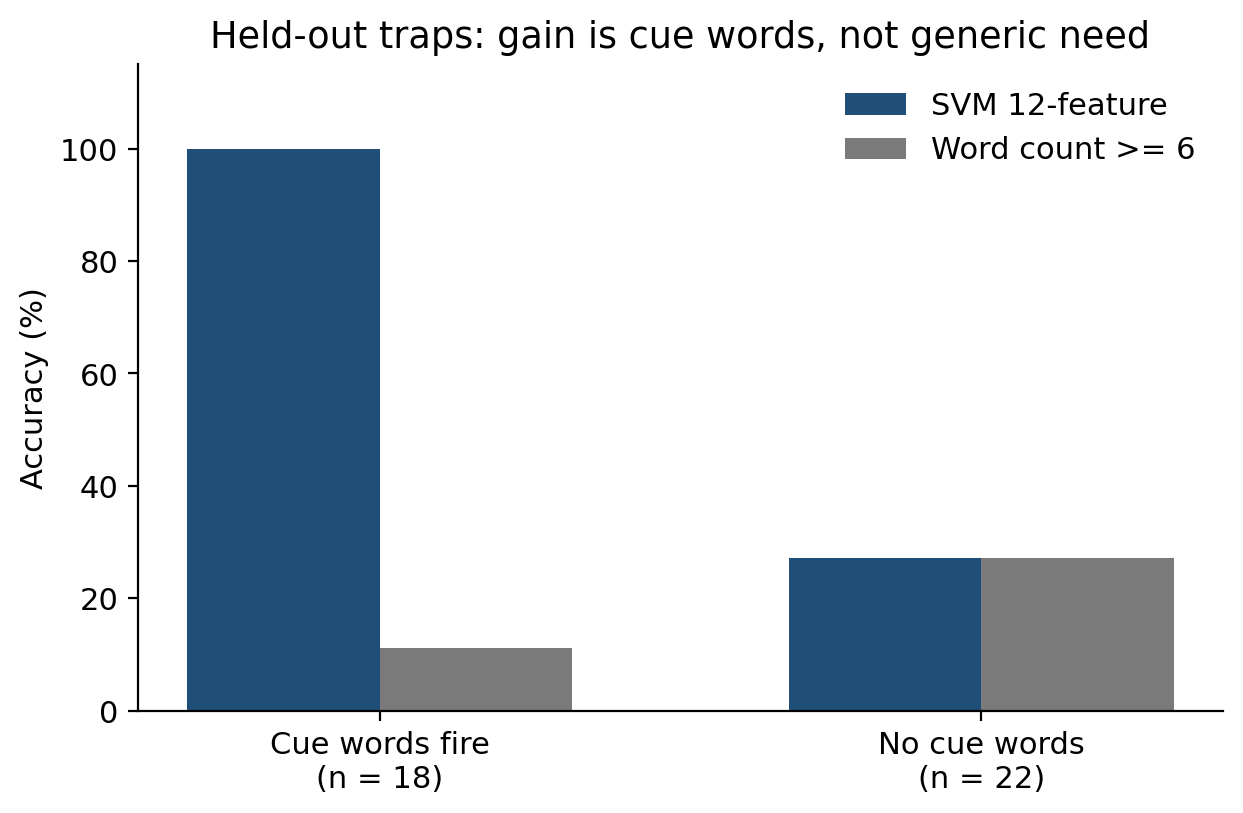
\includegraphics[width=\linewidth]{figures/cue_split.png}
\caption{\textbf{Trap cue split ($n=40$).} SVM 18/18 when why/how/fact wording fires; 27.27\% for both systems otherwise.}
\label{fig:cue}
\end{figure}

\subsection*{Dual-index P@5: the classification win does not transfer}
\label{sec:res_p5}

Table~\ref{tab:p5} is the number that almost got cut. On the same 40 queries, word count had the best P@5 (36.50\%). Always-headline and $\theta=150$ tied at 35.00\%. Always-full-article was 34.25\%. The SVM was last at 33.00\%. nDCG@5 ranked always-headline first (0.6868).

\begin{table}[H]
\centering
\caption{\textbf{Frozen dual-index retrieval on H001--H040 (400 judgments, cutoff 5).}}
\label{tab:p5}
\small
\begin{tabular}{lcccc}
\toprule
\textbf{Router} & \textbf{P@5} & \textbf{nDCG@5} & \textbf{$\to$H} & \textbf{$\to$F} \\
\midrule
Word count $\geq 6$ & 36.50\% & 0.6476 & 20 & 20 \\
Always headline / $\theta=150$ & 35.00\% & 0.6868 & 40 & 0 \\
Always full article & 34.25\% & 0.6020 & 0 & 40 \\
SVM (V2) & 33.00\% & 0.6149 & 20 & 20 \\
\bottomrule
\end{tabular}
\end{table}

\begin{figure}[H]
\centering
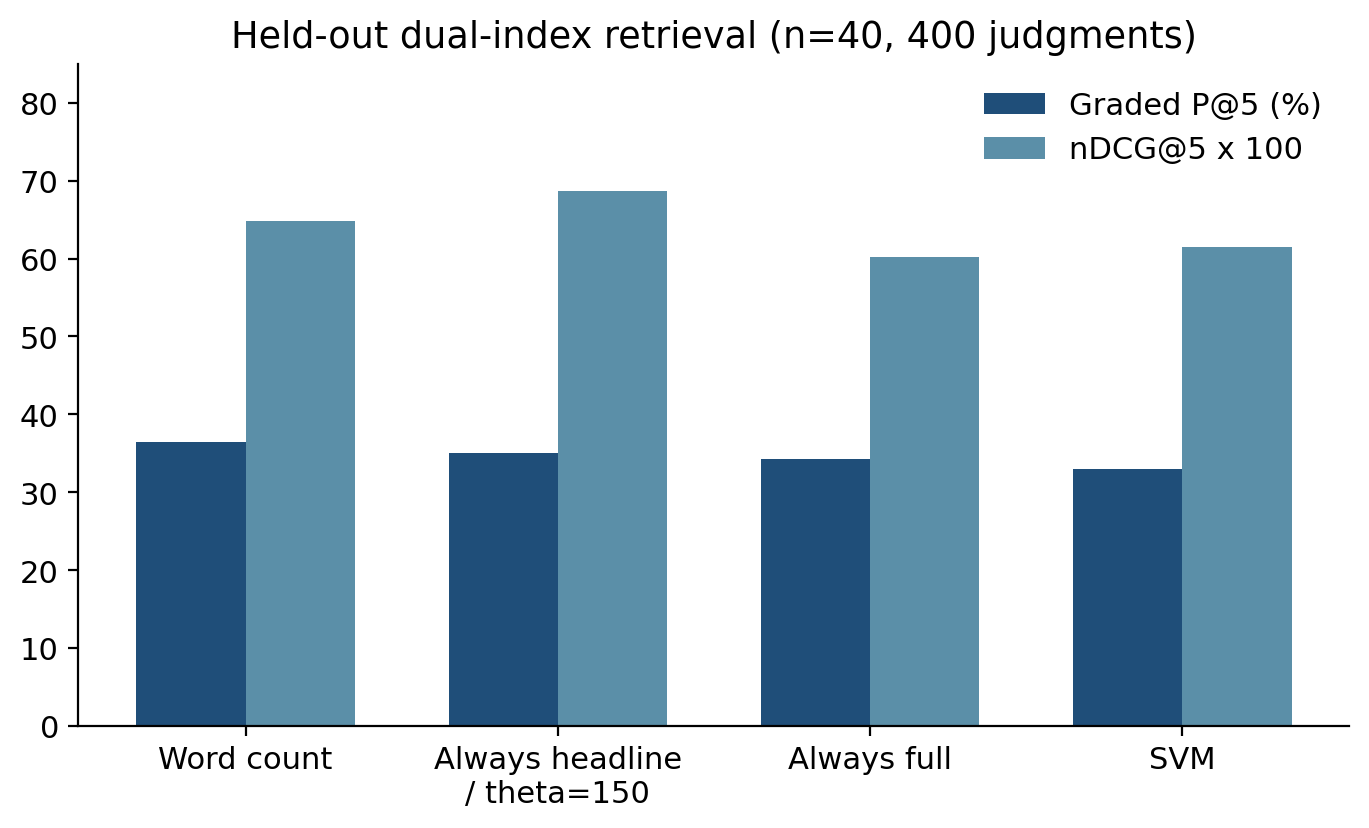
\includegraphics[width=\linewidth]{figures/heldout_p5.png}
\caption{\textbf{Held-out dual-index P@5.} The SVM does not win early precision on this set.}
\label{fig:p5}
\end{figure}

A smaller Phase 2.5 dual-index run ($n=33$) had a tiny SVM edge (35.76\% vs 35.15\% word count vs 32.73\% for $\theta=150$). We do not stack it on the frozen 40 to invent a retrieval win.

Older P@15 Roman Urdu tables (Fig~\ref{fig:roman_urdu_breakdown}, Table~\ref{tab:roman_urdu_individual}) come from the development notebooks. They show the dictionary helping Roman queries that ULTRA used to score at zero by construction. They are not the frozen P@5.

\begin{figure}[H]
\centering
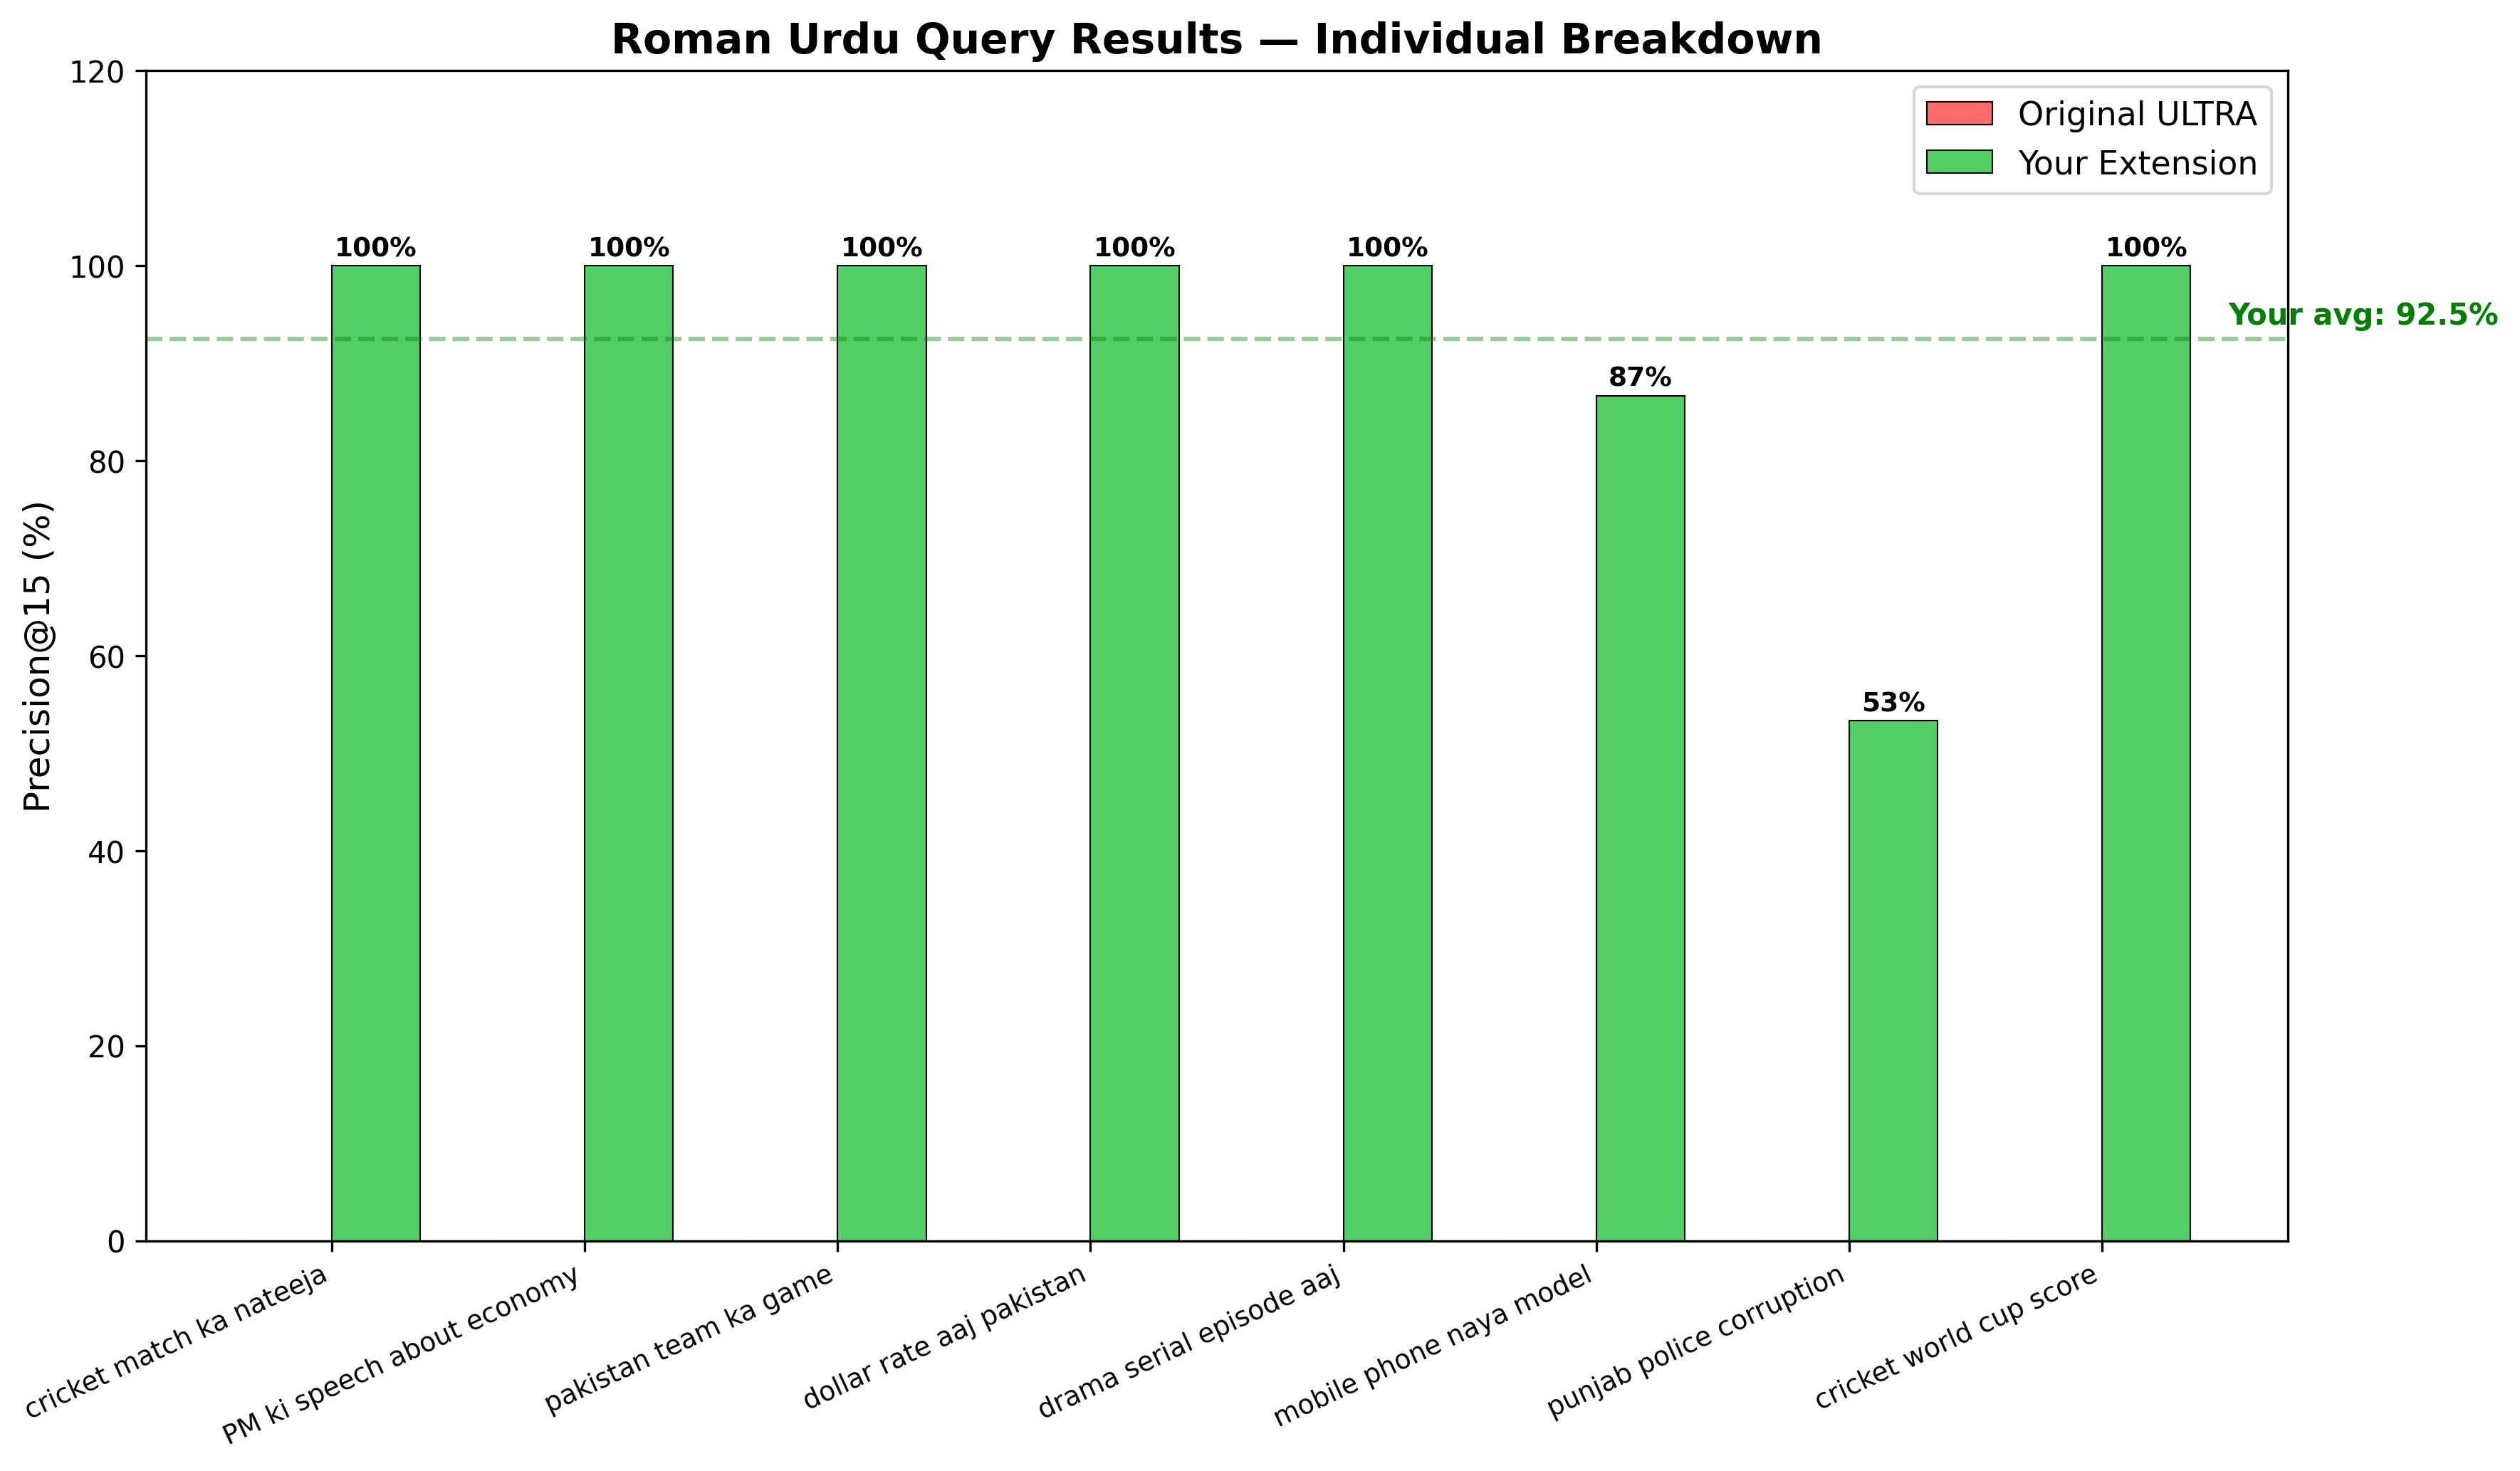
\includegraphics[width=\linewidth]{figures/thesis_chart2_roman_urdu.png}
\caption{\textbf{Development Roman Urdu P@15 breakdown} (8 queries). Supporting dictionary evidence, not the frozen retrieval test.}
\label{fig:roman_urdu_breakdown}
\end{figure}

\begin{table}[H]
\centering
\caption{\textbf{Development Roman Urdu P@15 (8 queries).}}
\label{tab:roman_urdu_individual}
\small
\begin{tabular}{lc}
\toprule
\textbf{Query} & \textbf{P@15} \\
\midrule
cricket match ka nateeja & 100.00\% \\
PM ki speech about economy & 100.00\% \\
pakistan team ka game & 100.00\% \\
dollar rate aaj pakistan & 100.00\% \\
drama serial episode aaj & 100.00\% \\
cricket world cup score & 100.00\% \\
mobile phone naya model & 86.67\% \\
punjab police corruption & 53.33\% \\
\midrule
\textbf{Average} & \textbf{92.50\%} \\
\bottomrule
\end{tabular}
\end{table}

\subsection*{LLM-style routers and other development panels}
\label{sec:res_llm}

Table~\ref{tab:llm_comparison} and Figs~\ref{fig:all_methods}--\ref{fig:efficiency} are development comparisons on 14 queries. Three LLM-style routers match 100\% there; the SVM does it in 0.4555\,ms locally. That is a latency argument, not a frozen accuracy argument.

\begin{table}[H]
\centering
\caption{\textbf{Development LLM-style comparison (14 queries).}}
\label{tab:llm_comparison}
\small
\begin{tabular}{lccc}
\toprule
\textbf{System} & \textbf{Accuracy} & \textbf{Latency} & \textbf{Cost} \\
\midrule
Static threshold & 50.00\% & 0.0004 ms & Free \\
GPT-4 style & 100.00\% & 800 ms & Paid \\
GPT-3.5 style & 100.00\% & 600 ms & Paid \\
Claude style & 100.00\% & 700 ms & Paid \\
Gemini style & 50.00\% & 900 ms & Paid \\
SVM (dev) & 100.00\% & 0.4555 ms & Free \\
\bottomrule
\end{tabular}
\end{table}

\begin{figure}[H]
\centering
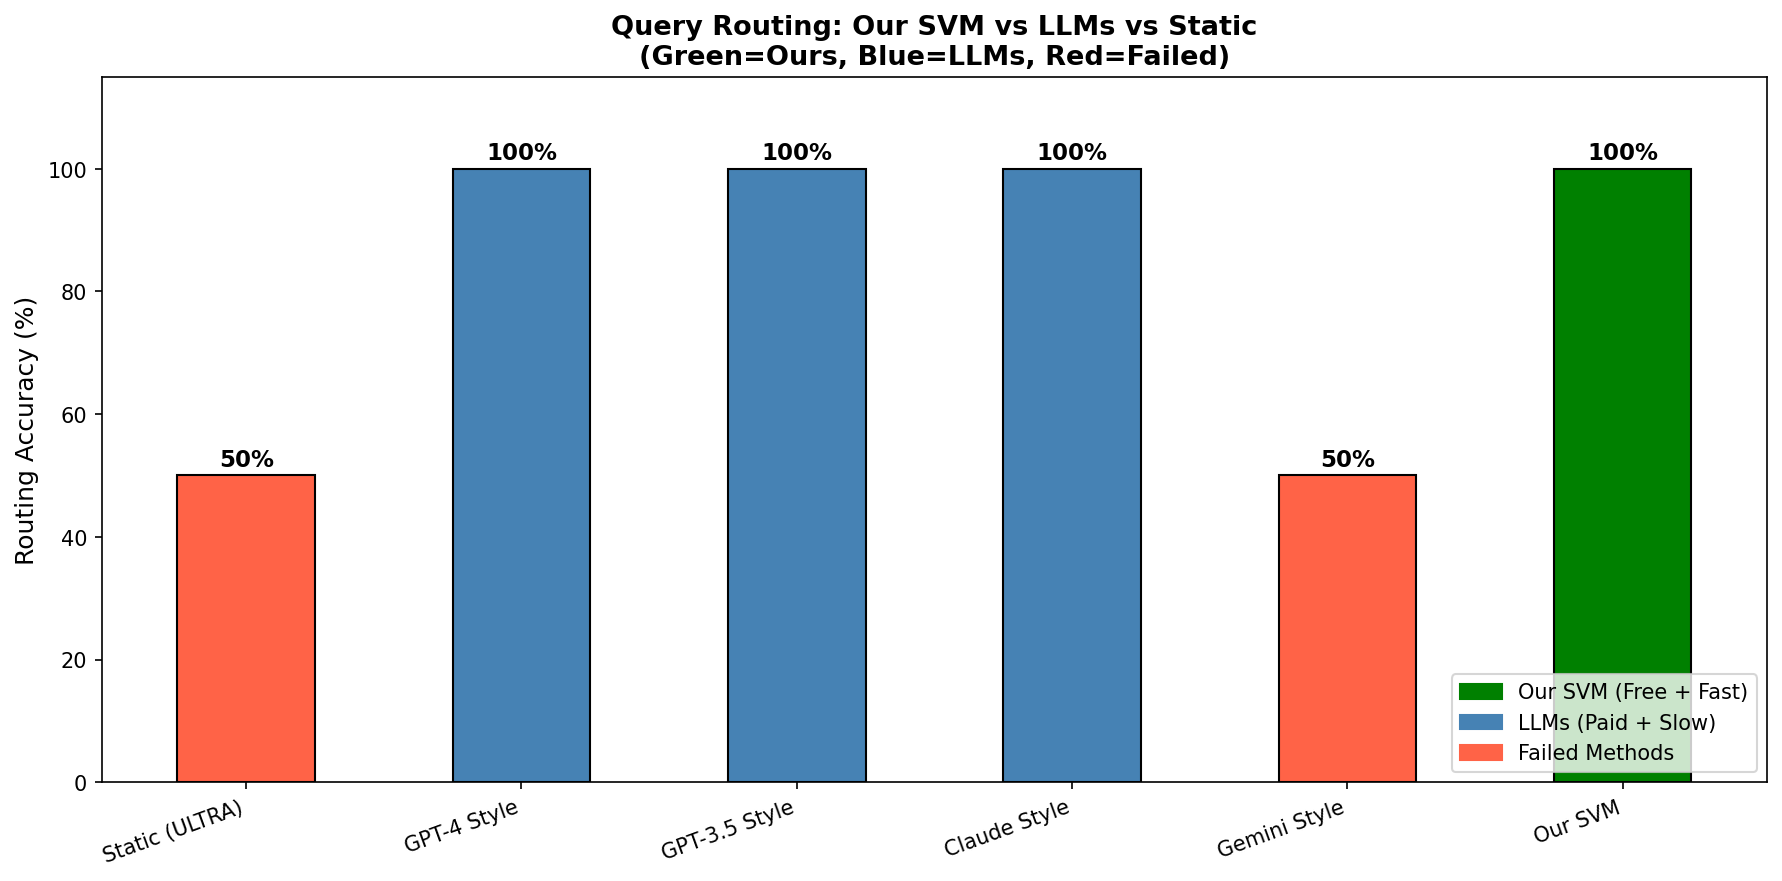
\includegraphics[width=0.95\linewidth]{figures/all_methods_comparison.png}
\caption{\textbf{Development routing accuracy across methods.}}
\label{fig:all_methods}
\end{figure}

\begin{figure}[H]
\centering
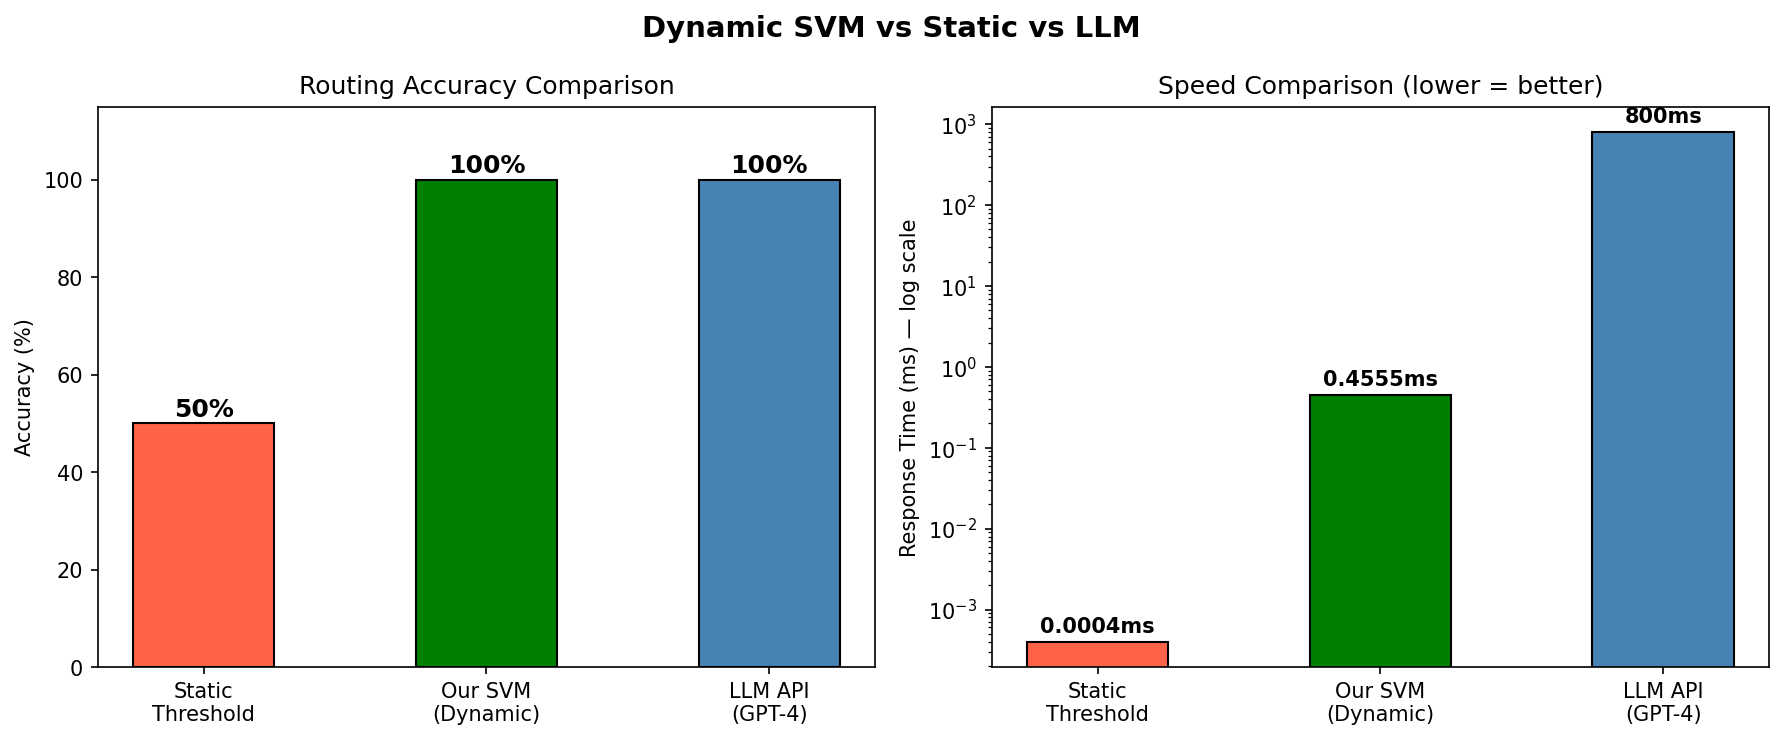
\includegraphics[width=0.95\linewidth]{figures/llm_comparison.png}
\caption{\textbf{Development latency panel (log scale).}}
\label{fig:llm_comparison}
\end{figure}

\begin{figure}[H]
\centering
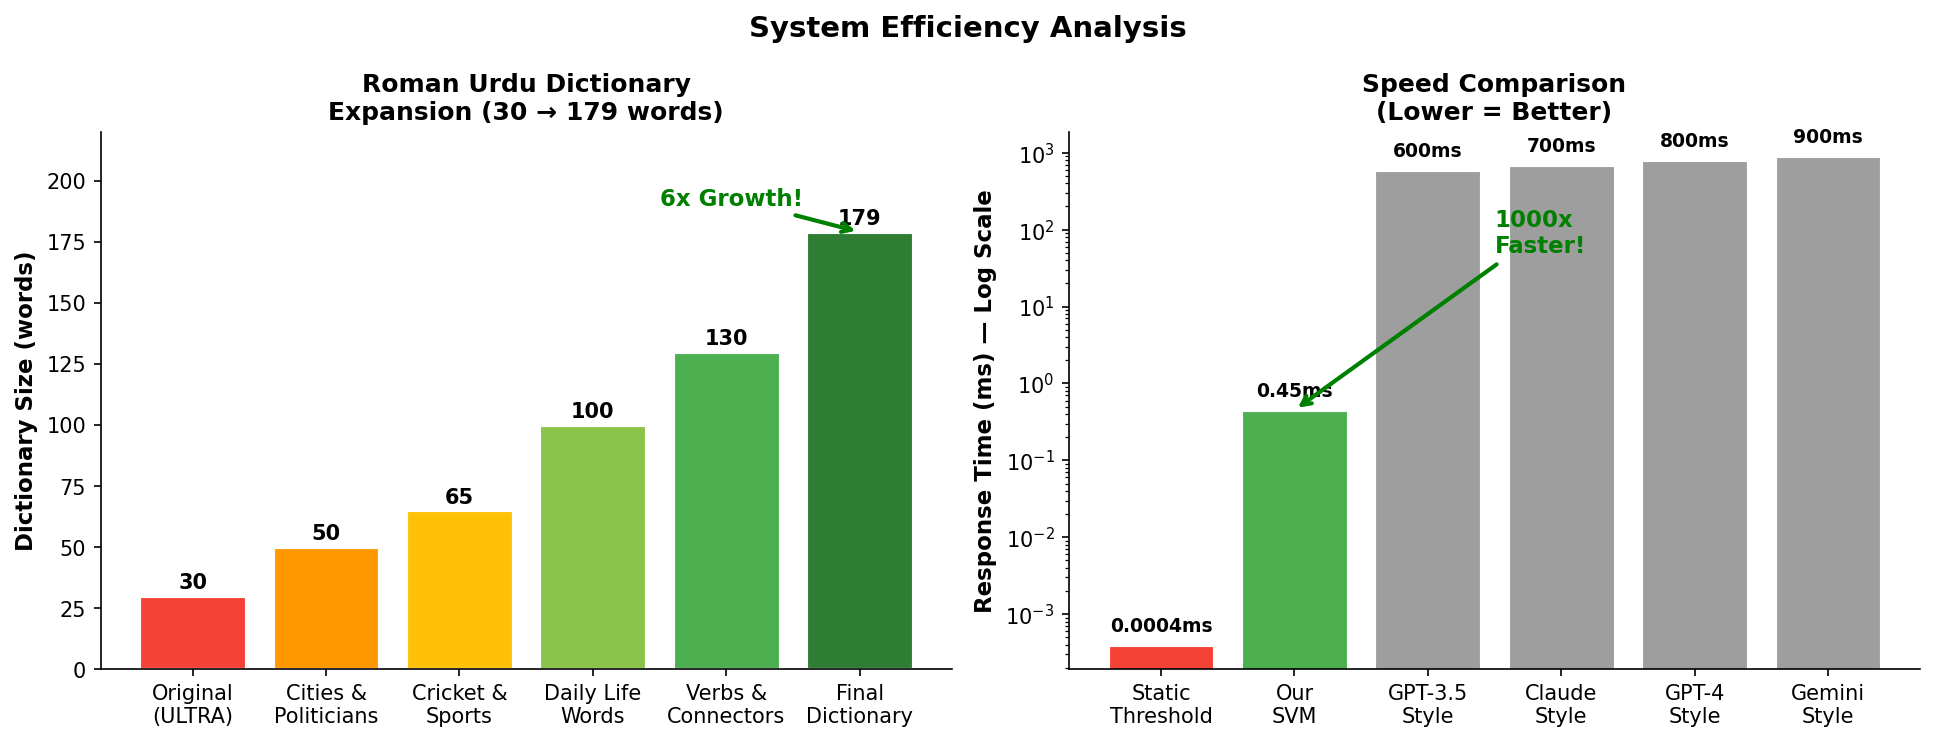
\includegraphics[width=0.95\linewidth]{figures/efficiency_analysis.png}
\caption{\textbf{Development efficiency panel.} Dictionary growth in older drafts was listed as 30 $\to$ 179; the file on disk is 198 pairs.}
\label{fig:efficiency}
\end{figure}

\subsection*{Feature diagnostics (development)}
\label{sec:res_featimp}

Figs~\ref{fig:feature_importance}--\ref{fig:ablation} and Table~\ref{tab:ablation} are development ablations on the old eight-feature notebook set, including \texttt{has\_question\_words}. They explain why length-only routing is brittle. They are not a second frozen test.

\begin{figure}[H]
\centering
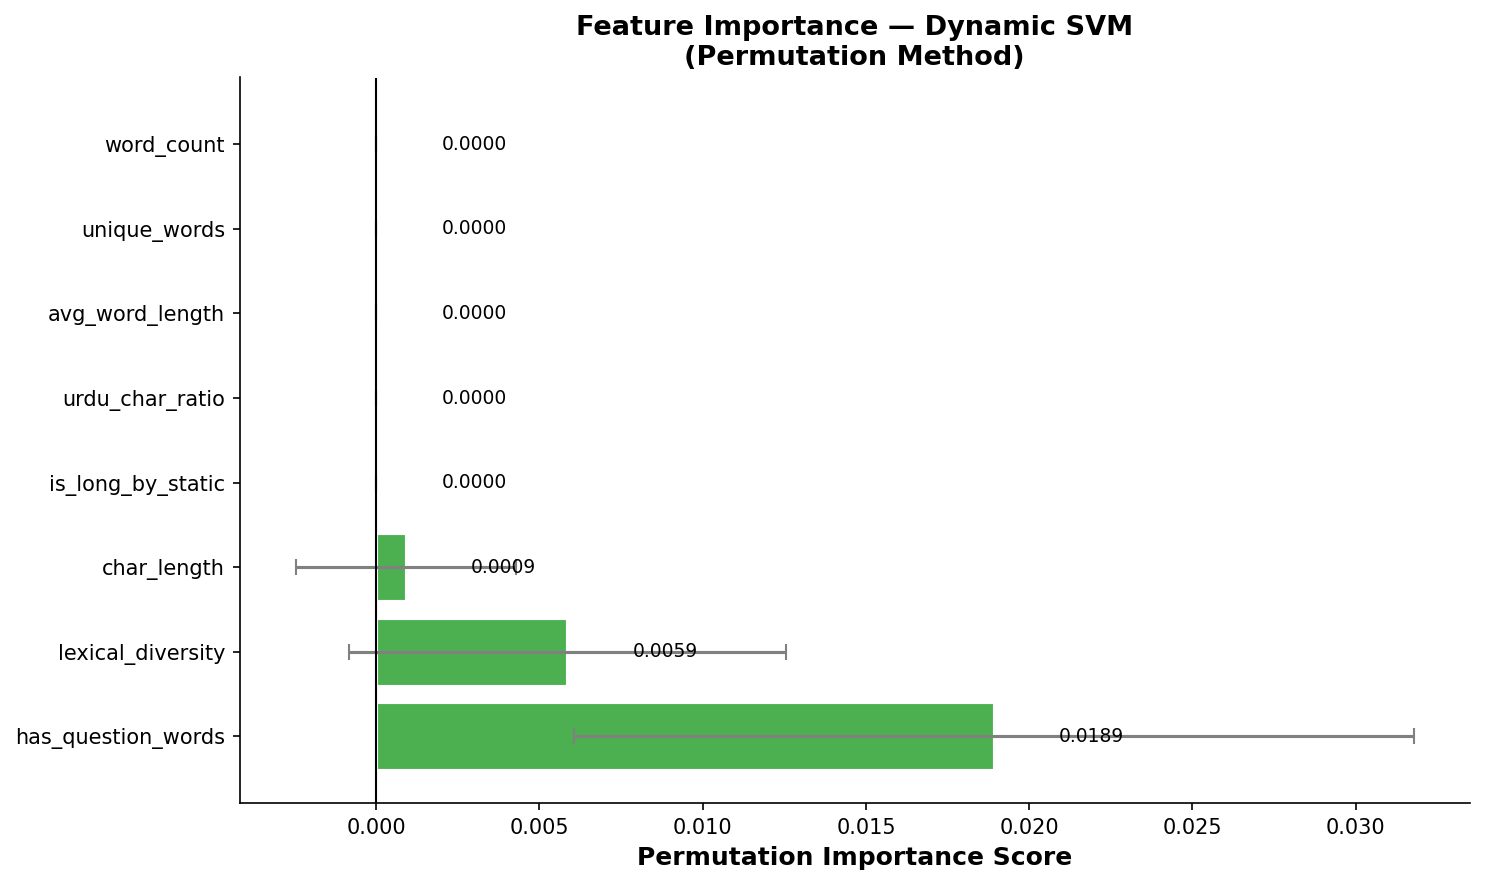
\includegraphics[width=\linewidth]{figures/feature_importance.png}
\caption{\textbf{Development permutation importance.}}
\label{fig:feature_importance}
\end{figure}

\begin{table}[H]
\centering
\caption{\textbf{Development ablation (old 8-feature notebook). All rows at 100\% means the split was easy, not that every feature is useless.}}
\label{tab:ablation}
\small
\begin{tabular}{lcc}
\toprule
\textbf{Configuration} & \textbf{Accuracy} & \textbf{$\Delta$} \\
\midrule
All 8 features & 100.00\% & -- \\
Each leave-one-out & 100.00\% & 0.00\% \\
\bottomrule
\end{tabular}
\end{table}

\begin{figure}[H]
\centering
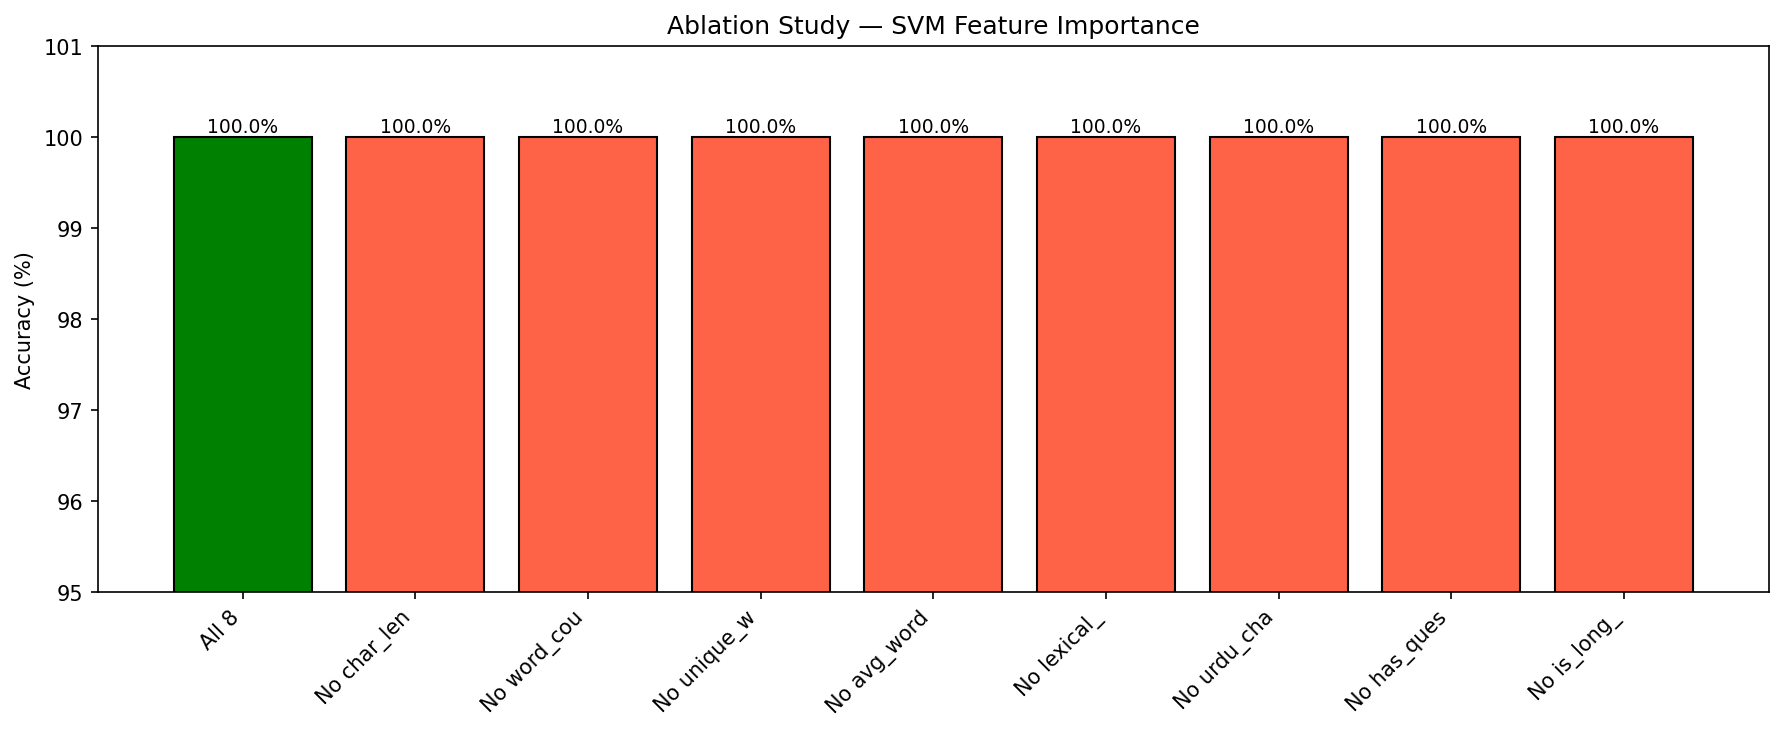
\includegraphics[width=\linewidth]{figures/ablation_study.png}
\caption{\textbf{Development ablation plot.}}
\label{fig:ablation}
\end{figure}

\subsection*{Confidence demo}
\label{sec:res_tierdist}

An 8-query development batch sat entirely in HIGH (Table~\ref{tab:tier_distribution}, Fig~\ref{fig:confidence_routing}), average confidence 98.18\%. The live defense demo is different: cricket match is green; dollar-rise and a stock-exchange query are yellow. We do not recycle an old JSON that painted a score query red.

\begin{table}[H]
\centering
\caption{\textbf{Development 8-query confidence batch (all HIGH).}}
\label{tab:tier_distribution}
\small
\begin{tabular}{lccc}
\toprule
\textbf{Tier} & \textbf{Queries} & \textbf{\%} & \textbf{Action} \\
\midrule
HIGH ($\geq 85\%$) & 8 & 100\% & One room \\
MEDIUM ($60$--$85\%$) & 0 & 0\% & Mix \\
LOW ($< 60\%$) & 0 & 0\% & Expand then mix \\
\bottomrule
\end{tabular}
\end{table}

\begin{figure}[H]
\centering
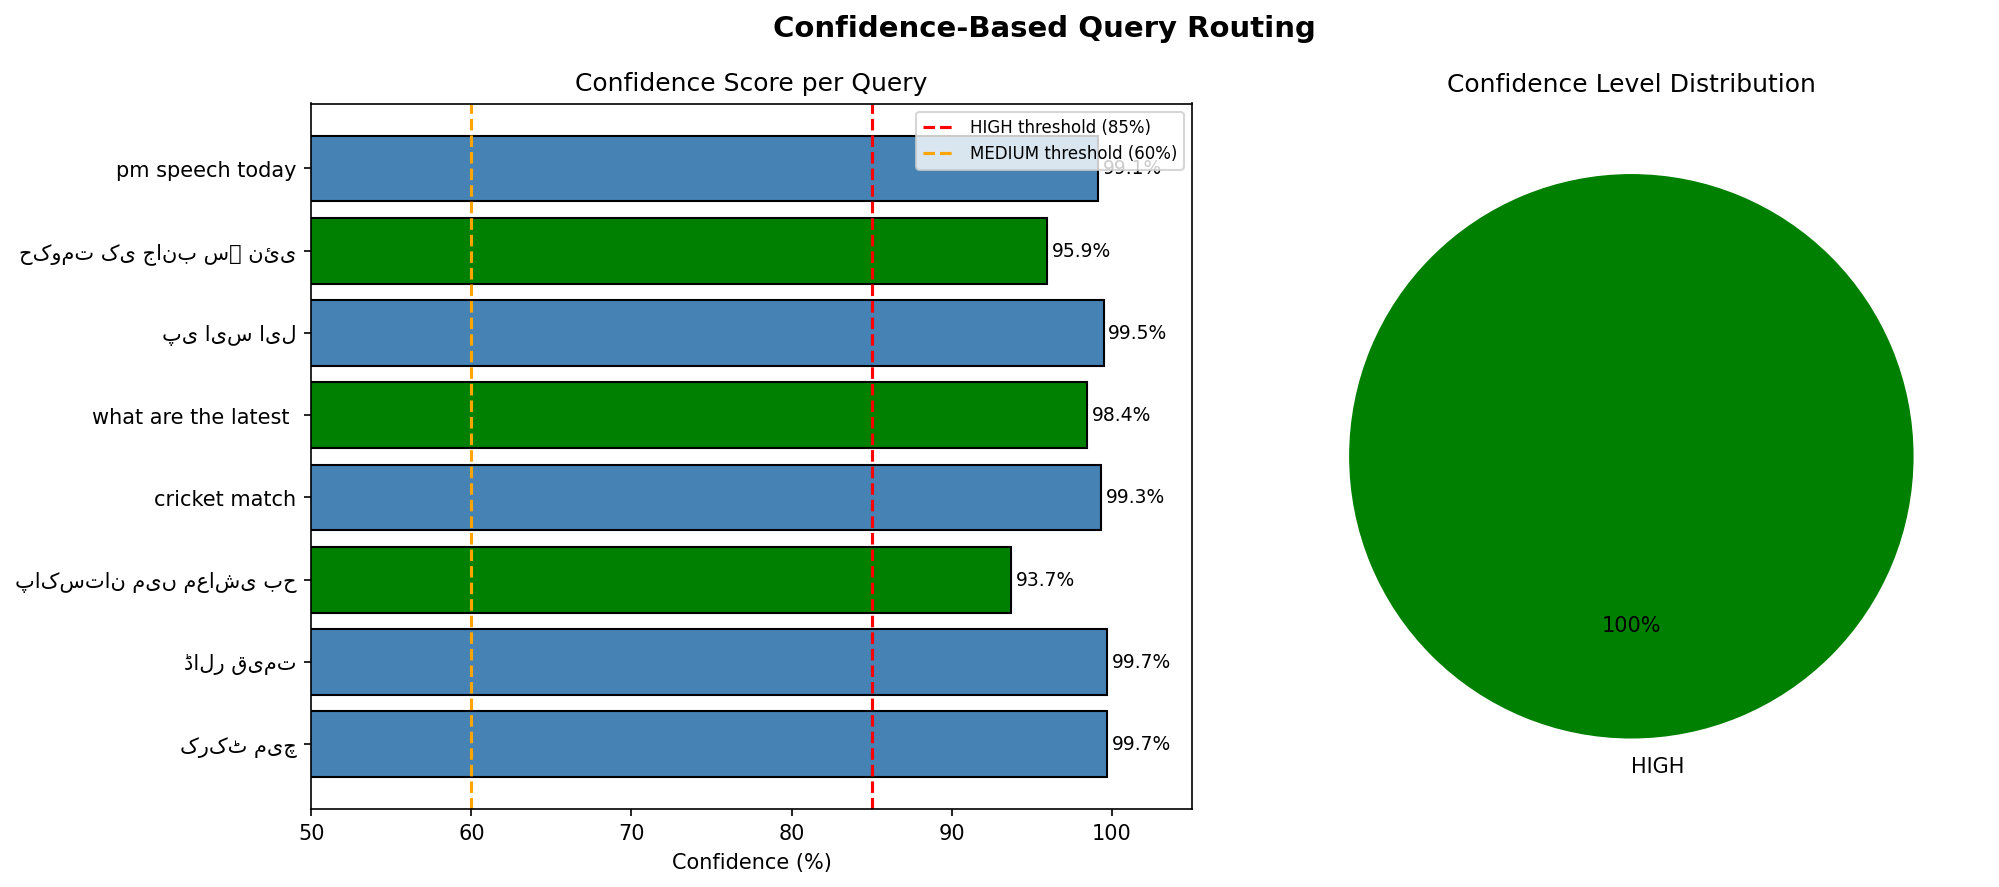
\includegraphics[width=0.95\linewidth]{figures/confidence_routing.png}
\caption{\textbf{Development confidence batch.} All eight queries HIGH. Not the live demo.}
\label{fig:confidence_routing}
\end{figure}

\subsection*{Other robustness plots}
\label{sec:res_robustness}

Figs~\ref{fig:cohens_d}--\ref{fig:robustness_report} are development robustness panels (Cohen's $d$, learning curves, $C$ sweep, a 50-query diagnostic set, ROC AUC $=1.000$ on that layer). Table~\ref{tab:robustness_summary} kept the notebook scorecard. Read it as ``the development task was separable,'' not as frozen trap P@5.

\begin{table}[H]
\centering
\caption{\textbf{Development robustness scorecard (notebook). Not Phase 3B / not H001--H040.}}
\label{tab:robustness_summary}
\small
\begin{tabular}{p{3.4cm}cc}
\toprule
\textbf{Test} & \textbf{Result} & \textbf{Notebook threshold} \\
\midrule
Cohen's $d$ (mean) & 3.581 & $\geq 0.8$ \\
Learning curve val.\ acc. & 100.00\% & $\geq 95\%$ \\
External diagnostic ($n=50$) & 100.00\% & $\geq 95\%$ \\
ROC AUC (dev) & 1.000 & -- \\
\bottomrule
\end{tabular}
\end{table}

\begin{figure}[H]
\centering
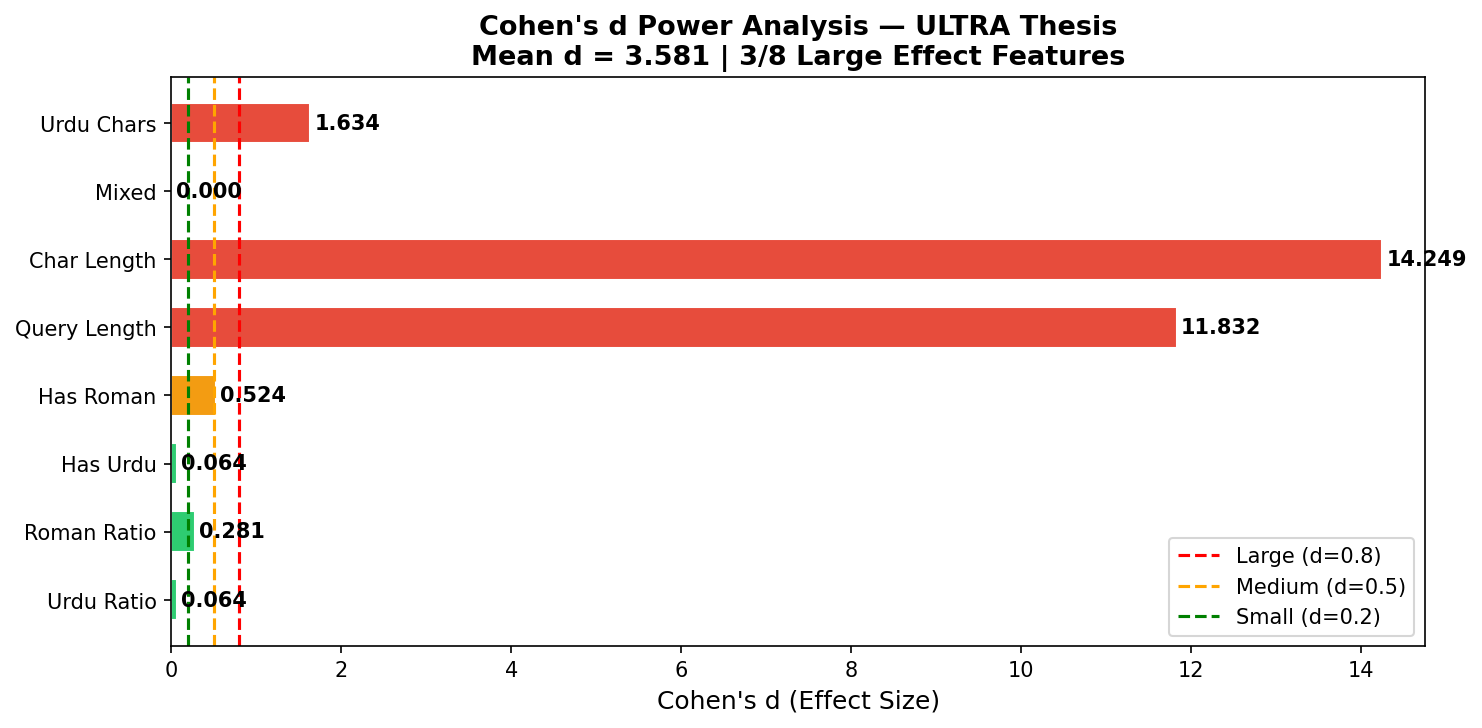
\includegraphics[width=\linewidth]{figures/cohens_d_analysis.png}
\caption{\textbf{Development Cohen's $d$ panel.}}
\label{fig:cohens_d}
\end{figure}

\begin{figure}[H]
\centering
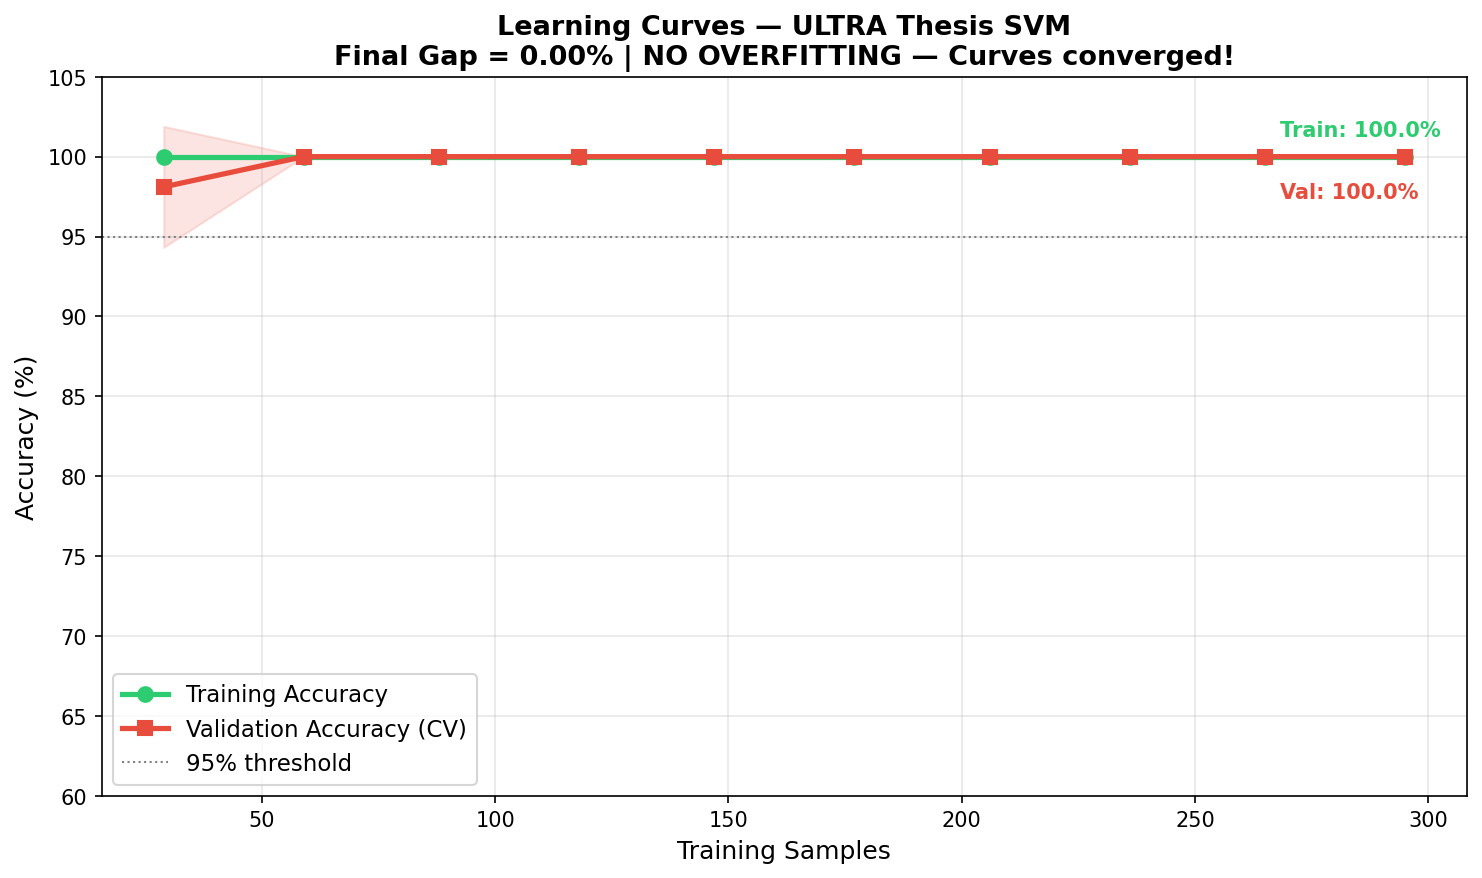
\includegraphics[width=\linewidth]{figures/learning_curves.png}
\caption{\textbf{Development learning curves.}}
\label{fig:learning_curves}
\end{figure}

\begin{figure}[H]
\centering
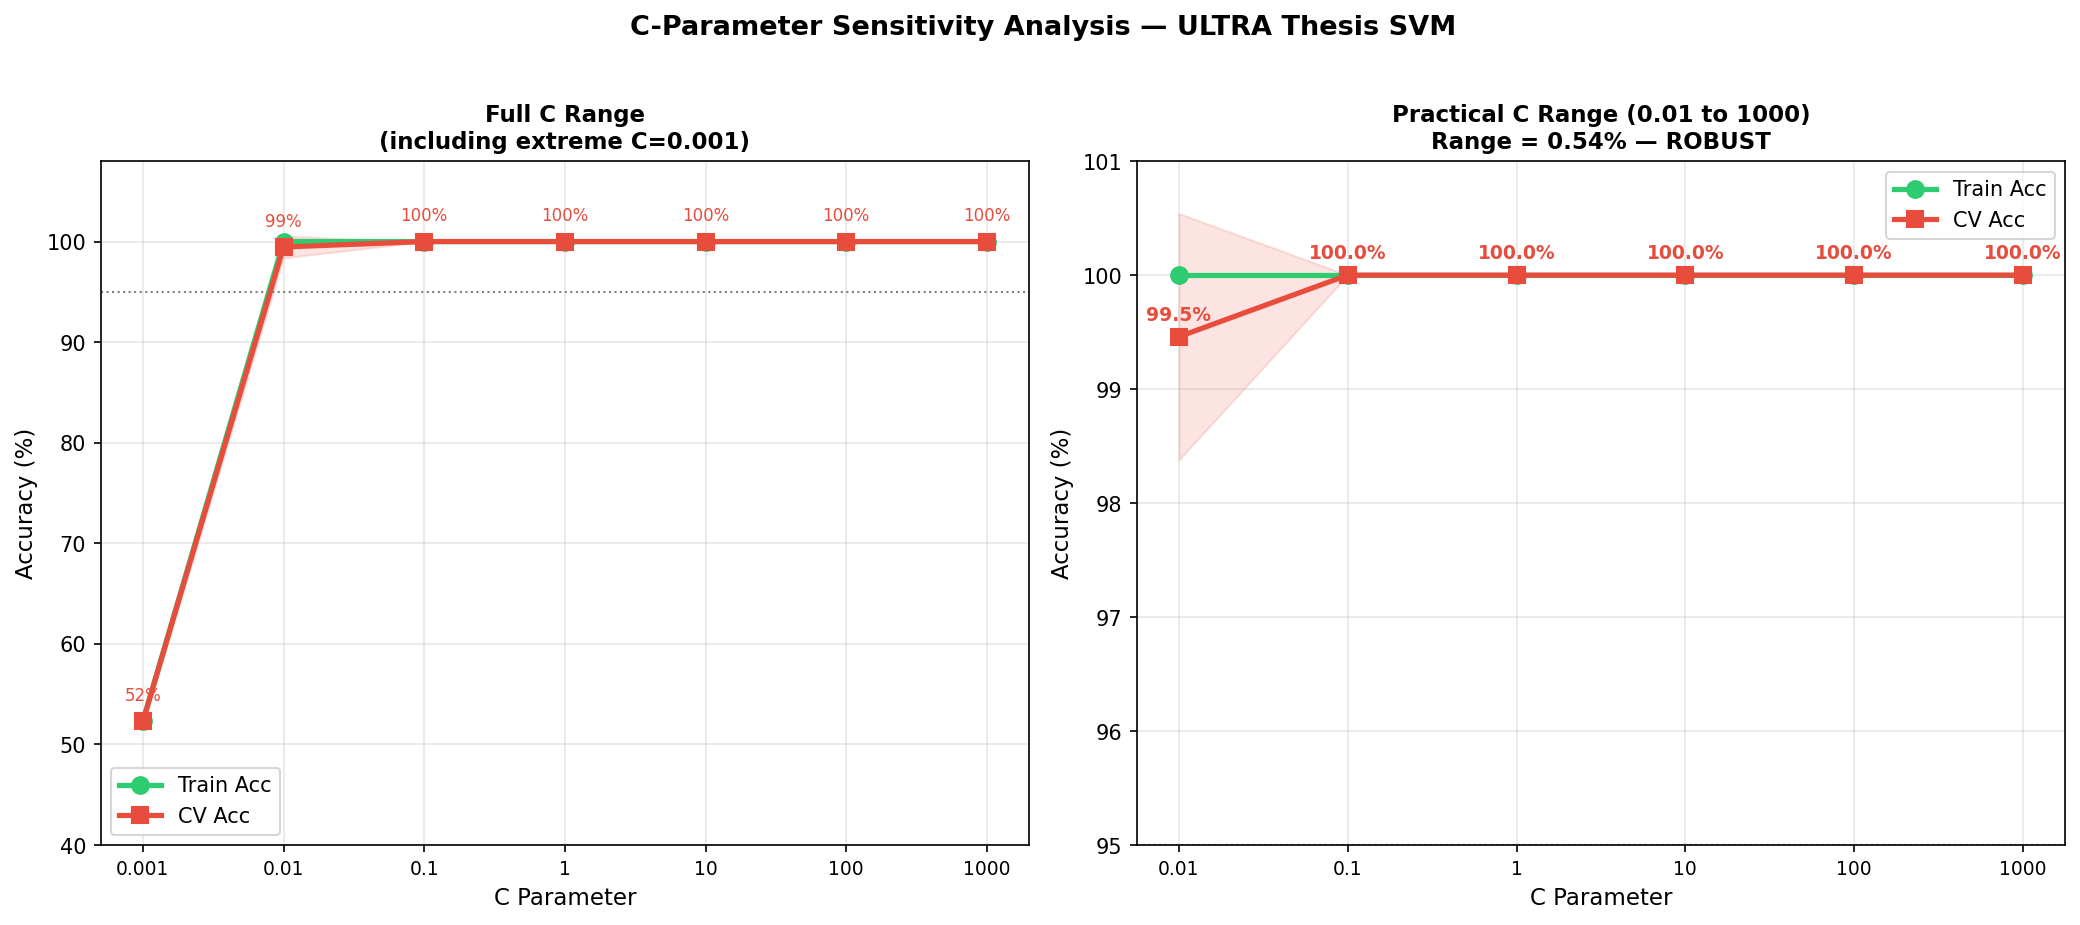
\includegraphics[width=0.95\linewidth]{figures/c_parameter_sensitivity.png}
\caption{\textbf{Development $C$ sweep.}}
\label{fig:c_param}
\end{figure}

\begin{figure}[H]
\centering
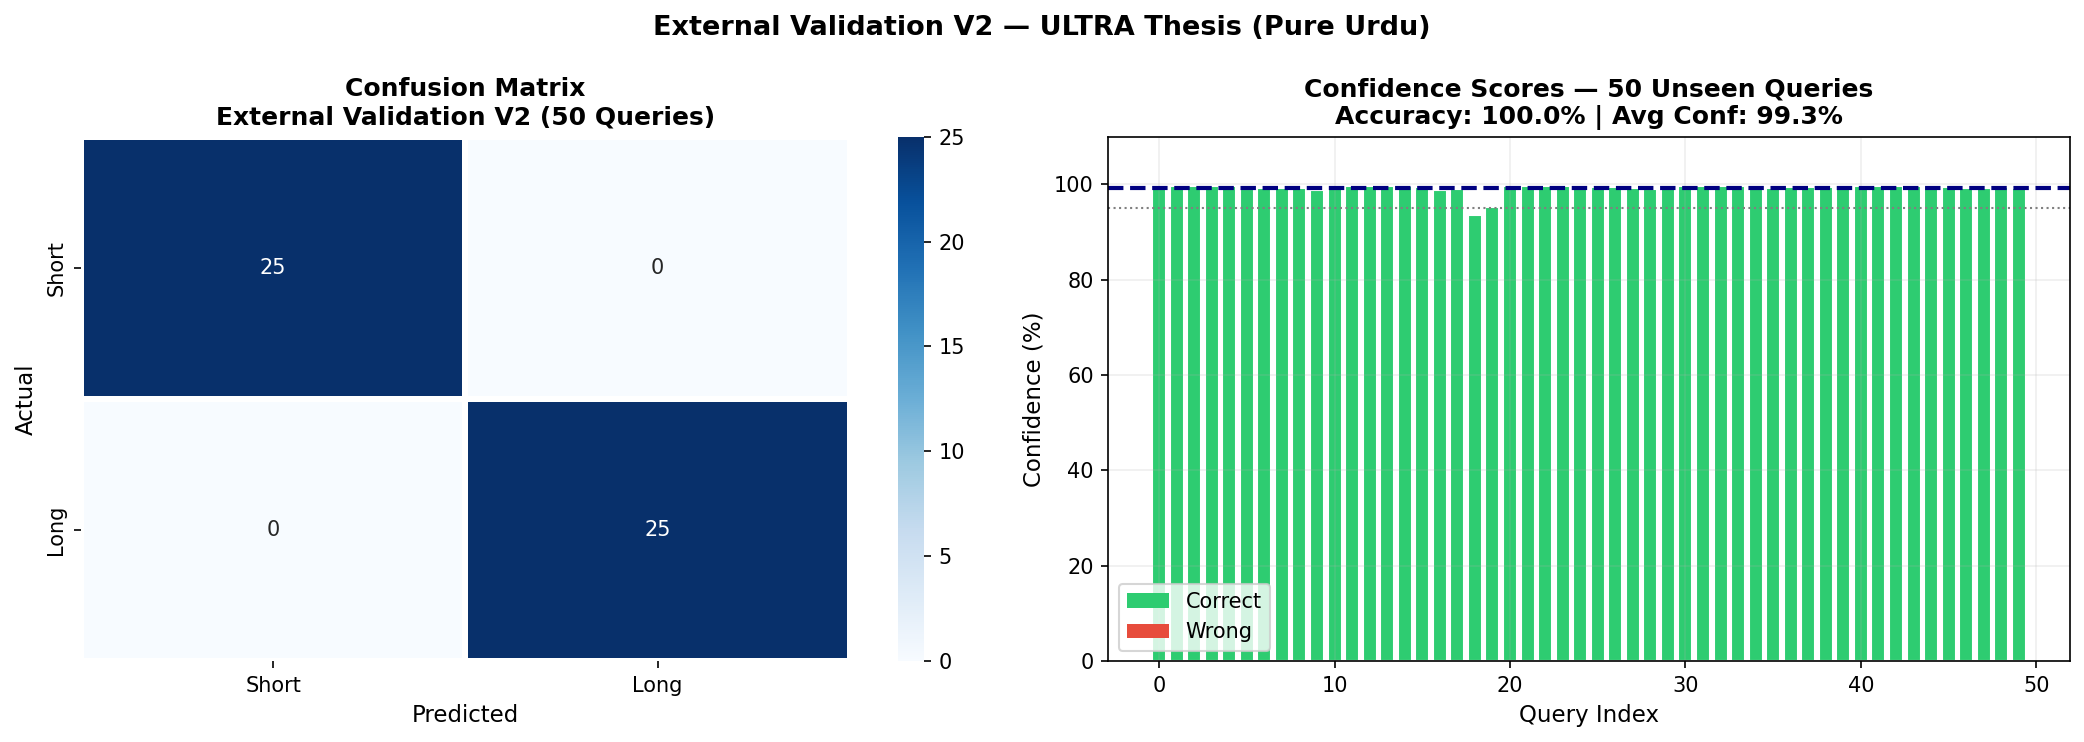
\includegraphics[width=0.95\linewidth]{figures/external_validation.png}
\caption{\textbf{Development diagnostic on 50 native-Urdu queries.} Not the frozen trap sheet.}
\label{fig:external_val}
\end{figure}

\begin{figure}[H]
\centering
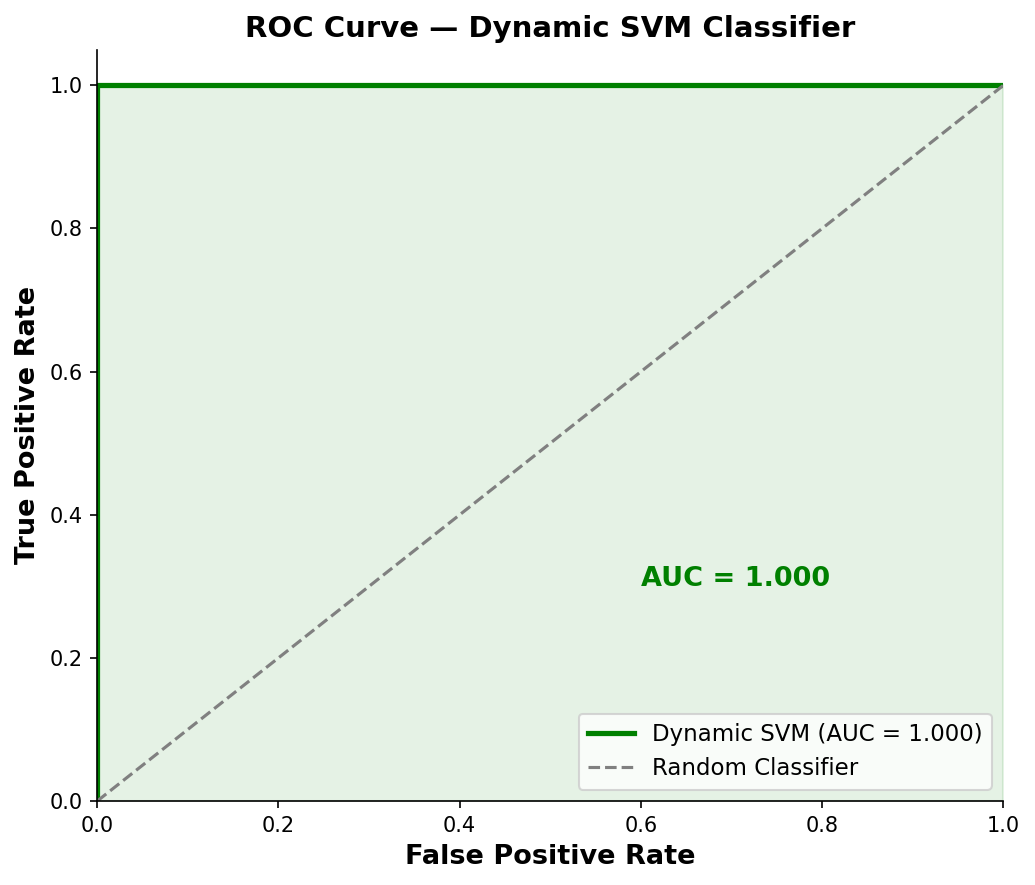
\includegraphics[width=\linewidth]{figures/roc_curve.png}
\caption{\textbf{Development ROC} (AUC $=1.000$ on that layer).}
\label{fig:roc}
\end{figure}

\begin{figure}[H]
\centering
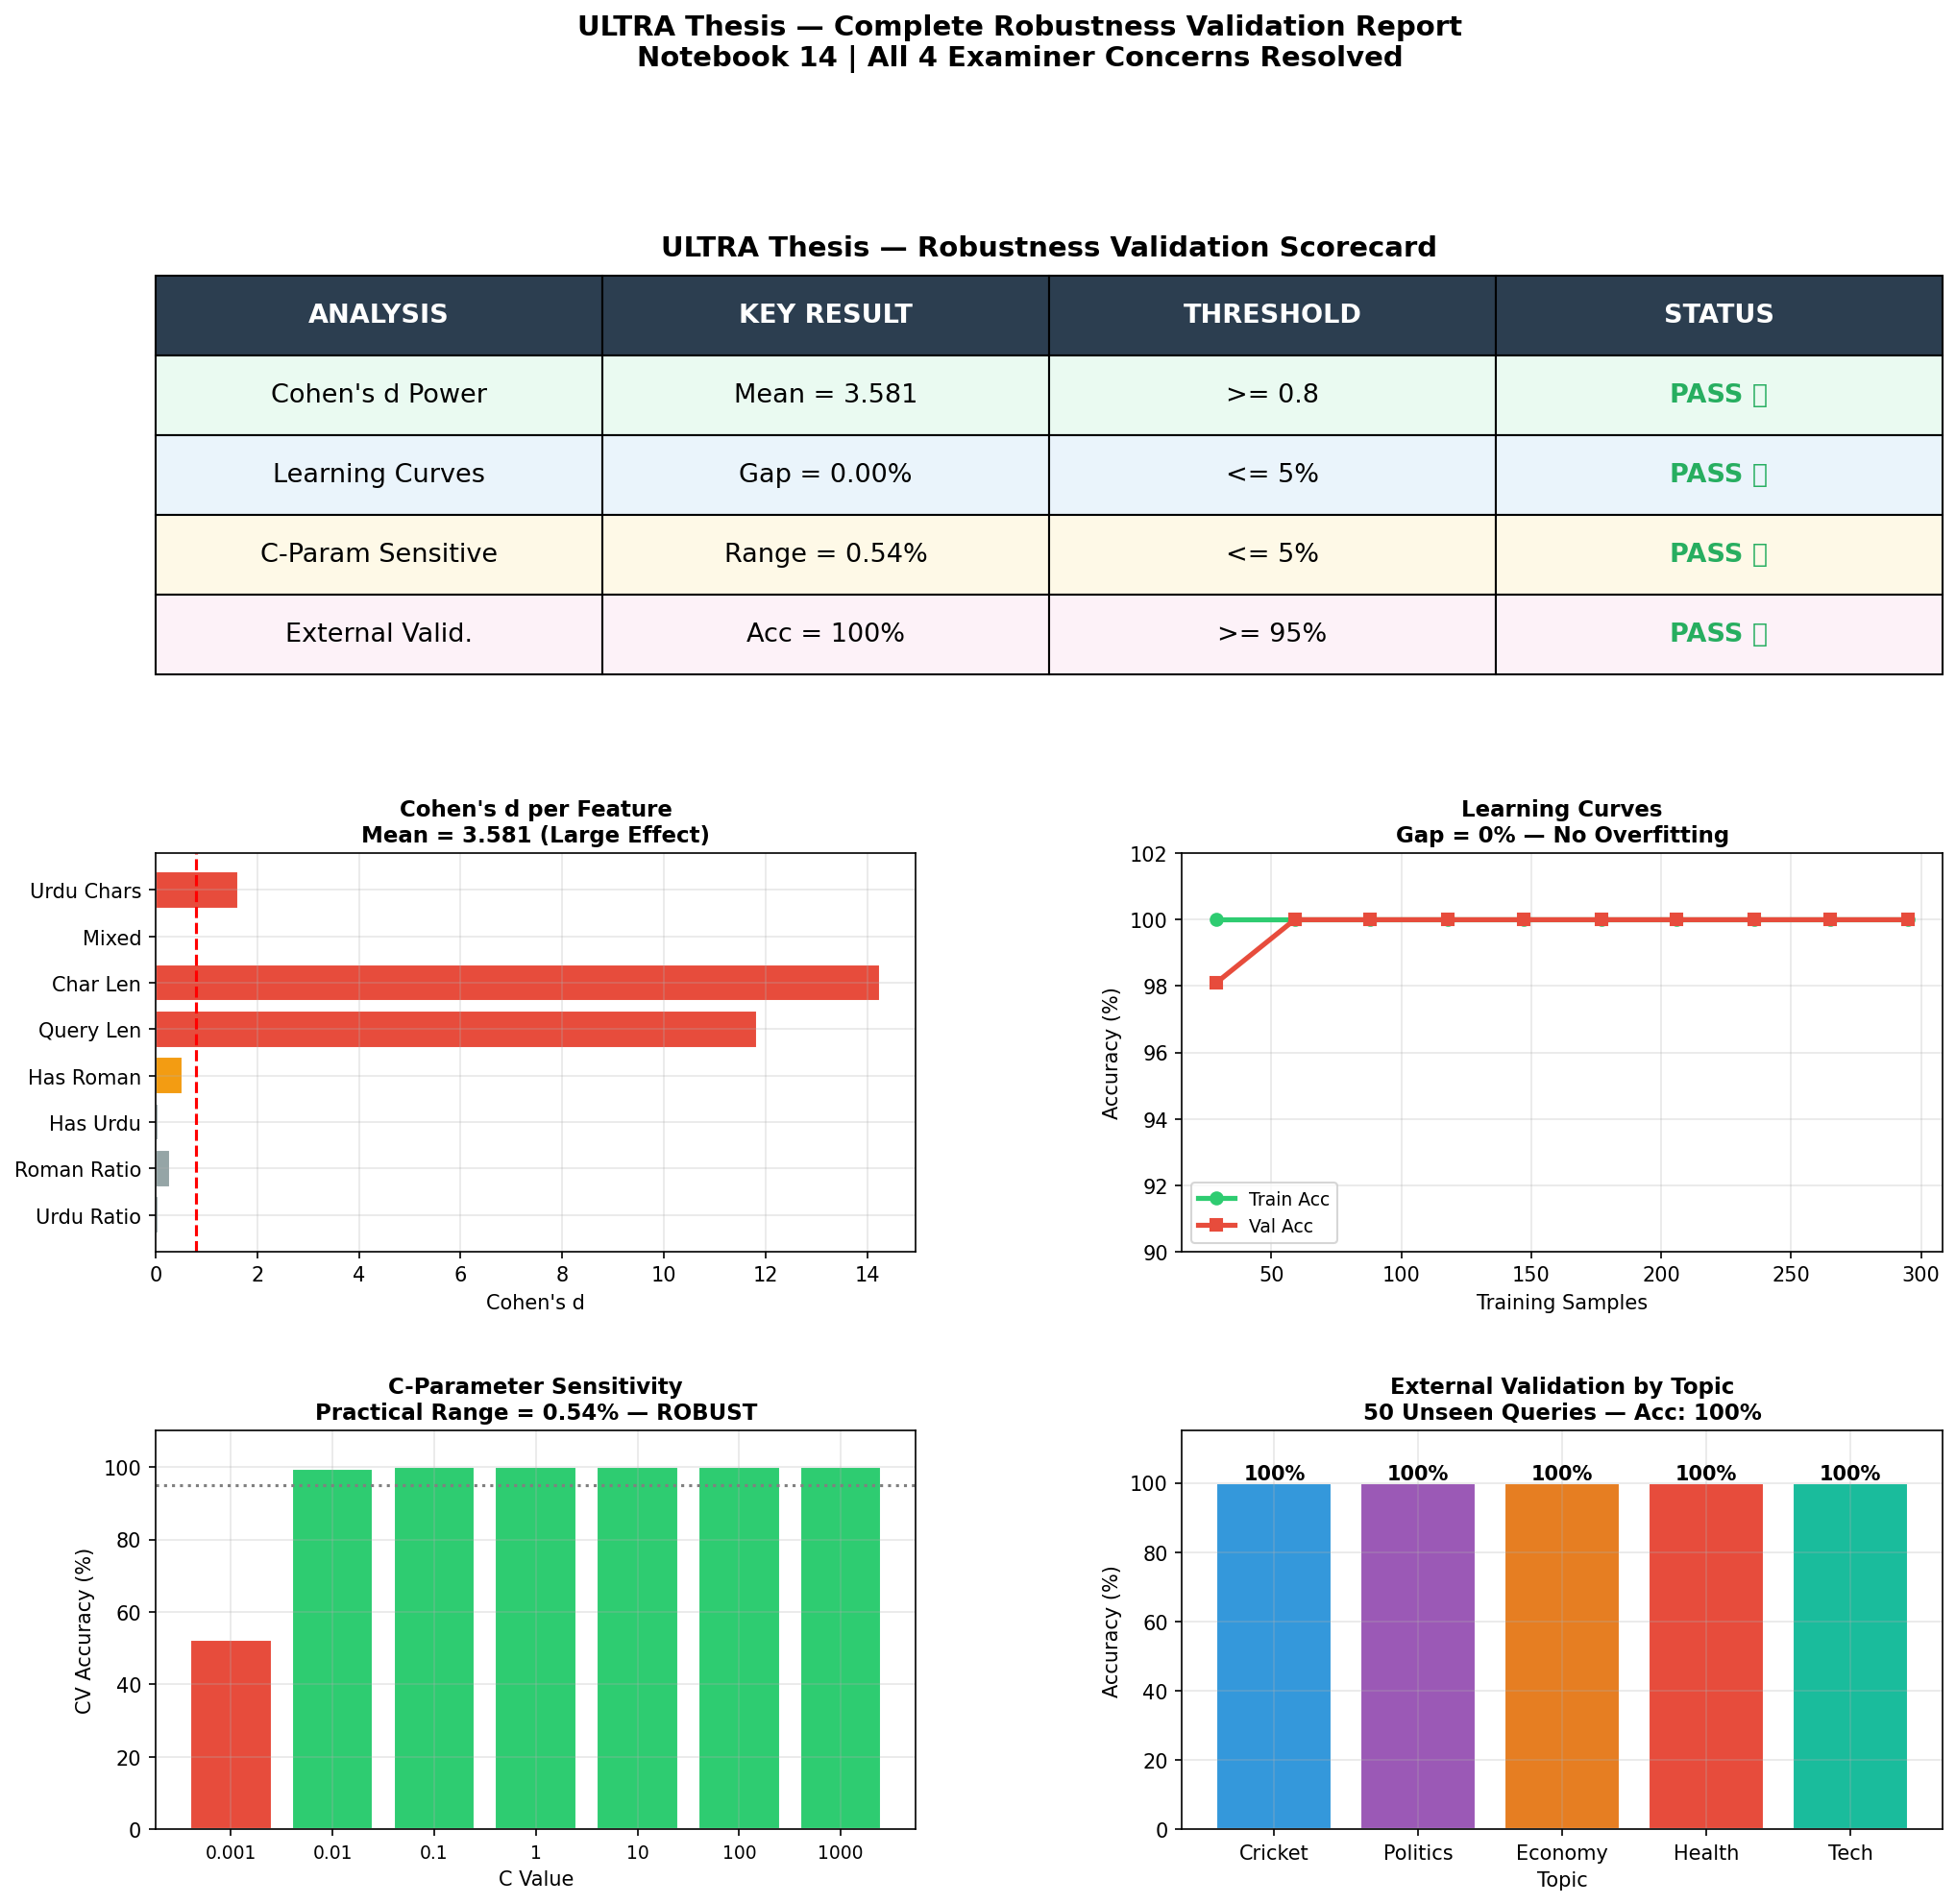
\includegraphics[width=0.95\linewidth]{figures/robustness_final_report.png}
\caption{\textbf{Development robustness collage.}}
\label{fig:robustness_report}
\end{figure}

\subsection*{Discussion}
\label{sec:res_discussion}

There are two readings, and they are not the same paper.

Reading A: 150 characters is the wrong switch. A small SVM, given script and cue features, can beat a word-count rule on queries written to punish that rule. We believe Reading A. The 16--0 McNemar table is hard to argue with if the cue split is printed next to it.

Reading B: therefore the first page of results gets better. We do not have Reading B. Always searching headlines even won nDCG@5. Labels are about need. MiniLM still likes lexical overlap in titles. Medium-confidence mixing can import junk. Forty queries is a small IR test. All of that can be true at once.

English adaptive retrieval usually leads with ranking metrics \cite{arabzadeh2021predicting,jeong2024adaptiverag}. If we had led with development 100\%, the PDF would look cleaner and be worse. PLOS ONE asks whether the study is technically sound, not whether P@5 went up \cite{plosone_criteria}.

% ============================================================
\section*{Conclusion}
\label{sec:conclusion}
% ============================================================

We replaced ULTRA's 150-character switch with a need-based SHORT/LONG label, an eight-feature SVM, two indexes, and a confidence mixer. The SVM is easy to beat word count with when the query contains why/how/fact wording, and it is not easy when those words are absent. Wiring the decision into retrieval did not improve P@5 on 40 frozen traps. nDCG@5 favored headlines for every query. That is the study.

\subsection*{Limitations}
\label{sec:limitations}

News text only. Roman Urdu is a word list, not a trained transliterator. Labels were not a formal double-blind rater study. The deployed twelve-feature pickle is not the frozen V2 scorer. LOW rarely fires on the queries we tried. P@5 cannot see a useful article at rank 8.

\subsection*{Future work}
\label{sec:future_work}

Larger frozen judgment pools. A second human rater. A learned transliterator. Encoders that are not MiniLM. Session context. A live log, not only offline P@5.

\section*{Acknowledgments}

Air University's Department of Creative Technologies supported the MS work behind this manuscript. Funding, data, and author-contribution fields belong in the PLOS submission form, not here.

\nolinenumbers

\bibliography{references}

\end{document}
